% !TEX root = main.tex
% !TeX encoding = UTF-8
% !TeX program = latexmk
% !TeX spellcheck = en_US

\documentclass[english,binding=0.6cm,noexaminfo]{sapthesis}

% --- PACKAGES ---
\usepackage[utf8]{inputenc}
\usepackage[english]{babel}
\usepackage{amsmath, amsfonts, amssymb, amsthm}
\usepackage{physics}
\usepackage{graphicx}
\usepackage{subcaption}
\usepackage{cite}
\usepackage{pgfplots}
\usepackage{bm}
\usepackage{float}
\usepackage[hidelinks]{hyperref}
\usepackage{microtype}
% --- MATHEMATICAL DEFINITIONS ---
\newcommand{\rhos}{\rho_s}
\newcommand{\vvec}{\mathbf{v}}
\newcommand{\jvec}{\mathbf{J}}
\raggedbottom
% --- METADATI DEL FRONTESPIZIO ---
\title{Non-reciprocal effects in two-dimensional \\superconductors studied by conformal mapping}
\subtitle{}
\author{Francesco Lupicuti}
\IDnumber{2141621} % Ricordati di inserire la tua matricola
\course{Bachelor's Degree in Physics} % Deve rimanere in italiano come da regolamento
\courseorganizer{Faculty of Mathematical, Physical and Natural Sciences}
\AcademicYear{2025/2026}
\advisor{Prof. Josè Lorenzana}
\authoremail{lupicuti.2141621@studenti.uniroma1.it} % Inserisci la tua email istituzionale
\copyyear{2026}
\thesistype{Bachelor's Degree Thesis}

% ==========================================
% TITLE PAGE
% ==========================================

\begin{document}

\frontmatter
\maketitle % FONDAMENTALE: questo genera fisicamente il frontespizio!
\dedication{A Cami, amica speciale. \\ Eri, sei e sarai sempre nel mio cuore.}
\tableofcontents

\mainmatter % Passa la numerazione delle pagine in numeri arabi
\chapter*{Introduction}
\markboth{Introduction}{} % Impedisce che in alto appaia "Indice" al posto di "Introduction" [cite: 815, 816]
\addcontentsline{toc}{chapter}{Introduction}

The study of two-dimensional (2D) superconducting systems represents one of the richest fields of investigation in condensed matter physics. This thesis contributes to this field developing methods to analyze non-reciprocal effects in superconducting devices. Specifically, we investigate the behavior of particular devices in the presence of an external current.
 The chosen mathematical approach relies on the formalism of complex analysis and conformal mapping, which allows for the rigorous modeling of the superconductor and its transport properties via a complex potential.

A crucial physical problem addressed in this work concerns the stability of the superconductor in the vicinity of topological defects known as vortices. A superconducting vortex is characterized by a persistent current circulating in a certain direction around the normal region. Consider a single vortex strongly pinned in some place due to some artificial means, such as impurities or a physical core in the material: when an external current is applied, the spatial symmetry of the flow around the defect is broken. In specific regions near the edges, the superfluid velocity field becomes locally larger. If the kinetic energy of the currents exceeds a specific critical threshold—dictated by the Cooper pair \textit{depairing} velocity—the material locally loses its superconducting properties and transitions into the normal, dissipative state.

Mathematically, this phase boundary is described by a specific line of the velocity field: the locus of points where the squared velocity reaches its critical value. The fundamental observation driving this analysis is that, in the presence of external currents, this critical line deforms and shifts relative to the original physical edge of the defect. Consequently, the effective "obstacle" perceived by the superconductor is no longer the original normal region, but a deformed one. This geometric deformation subsequently alters the global current distribution, dictating that the entire boundary-value problem must be solved self-consistently.

To capture this complex phenomenology, this work 
proposes different schemes. 
 Once the deformation of the critical line in the perturbed system is analyzed, the corrections developed in this work aim to mitigate the non-self-consistency by spatially adjusting the boundary of the normal region to accommodate the new profile. This geometric self-adjustment allows for an approximate tracing of the actual boundary of the region where superconductivity effectively survives.

%However, since modifying the physical boundary inherently alters the boundary conditions of the system, the entire velocity field reorganizes, giving rise to a new critical line. For this reason,

A complete spatial correction procedure should ideally be implemented as a continuous iterative process. In this thesis, the scope of the analysis is restricted to the first iteration of this hypothetical self-consistent computation. We focus on two configurations: a single vortex and a dipole (i.e., a vortex-antivortex pair with current circulating in opposite directions). Interestingly, for the dipole configuration, one can see the emergence of non-reciprocal effects, such as the superconducting diode effect.\\ 
The thesis is organized as follows: Chapter 1 reviews the theoretical foundations of two-dimensional superconductivity and topological transitions. Chapter 2 introduces the mathematical formalism of conformal mapping. Chapter 3 outlines the theoretical model, geometric feedback approximations, and computational results for a single pinned vortex. Chapter 4 extends this framework to the dipolar configuration (vortex-antivortex pair), analyzing its phase diagram and the emergence of the superconducting diode effect. Finally, Chapter 5 summarizes the conclusions and outlines future perspectives.\\
The numerical programs developed for this work are contained in the \textit{Wolfram Mathematica} notebook \texttt{2D-Superdiode.nb}\footnote{\url{https://github.com/Lupicuti/2D-Superdiode}}. In general terms, the code implements the formalism of conformal mappings to analytically calculate and numerically visualize the "current textures" in the superconductor and analize the breakdown points of the superconducting phase as a function of external parameters like the applied current.
% ==========================================
% CHAPTER 1: XY MODEL AND TOPOLOGICAL TRANSITIONS
% ==========================================
\chapter{Ginzburg-Landau Theory and XY Model}
\label{cap:physicsframework}
\section{The Ginzburg-Landau Theory in two dimensions}

Firstly, it is useful to establish why a macroscopic quantum system like a superconductor can be described by a single continuous field, especially at absolute zero temperature ($T=0$ K). 

Because electrons are fermions subject to the Pauli exclusion principle, they must occupy distinct quantum states, sequentially filling the lowest available energy levels to form a dense "Fermi sea." The maximum energy level reached in this ground state is the Fermi energy, and the boundary in momentum space separating occupied from unoccupied states constitutes the Fermi surface. According to the microscopic Bardeen-Cooper-Schrieffer (BCS) theory \cite{bardeen1957theory,cooper1956bound}, the superconducting phase transition at extremely low temperatures is driven entirely by the dynamics of electrons in the immediate vicinity of the Fermi surface. Electrons deep within the "Fermi sea" are kinematically locked; any scattering event or interaction would require them to transition into an already occupied state, which is quantum-mechanically forbidden. Consequently, only those electrons residing directly at the Fermi surface---where infinitesimally higher, unoccupied energy states are readily available---possess the necessary degrees of freedom to scatter and interact. As these energetic surface electrons travel through the crystal lattice, they slightly displace the heavier, positively charged ions along their path. This creates a delayed, localized region of enhanced positive charge---a phonon "wake." A second electron is then attracted to this wake, resulting in a net effective attraction that overcomes their natural Coulomb repulsion. This phonon-mediated interaction causes them to bind together into pairs with opposite momenta and spins, known as Cooper pairs. Because a Cooper pair consists of two half-integer spin fermions, it behaves effectively as a composite boson with an integer spin (typically $S=0$ in conventional $s$-wave superconductors).

Being bosonic in nature, Cooper pairs are not subject to the Pauli exclusion principle. As the temperature approaches $T=0$ K and thermal fluctuations vanish, all the pairs undergo a phase transition analogous to Bose-Einstein condensation, collapsing into the exact same quantum ground state. Consequently, the individual microscopic degrees of freedom are lost, and the ensemble of pairs (on the order of Avogadro's number ($\approx 10^{23}$ particles)) acquires macroscopic quantum coherence; therefore, it can be perfectly described by a single macroscopic wave function (or complex order parameter):
\begin{equation}
    \psi(\vec{r}) = \sqrt{\rho(\vec{r})} e^{i\theta(\vec{r})}
\end{equation}
where the square of the amplitude, $\rho(\vec{r}) = |\psi(\vec{r})|^2$, represents the physical local density of the Cooper pairs. The most crucial feature of this condensed state is governed by the phase $\theta(\vec{r})$: instead of exhibiting random, destructively interfering quantum phases like electrons in a normal metal, all Cooper pairs "lock" their phases together into a single, coherent macroscopic phase. This phase rigidity across macroscopic distances is the ultimate source of quantum coherence; it protects the condensate from individual particle scattering and dictates that any spatial phase gradient ($\nabla\theta$) will drive a collective, dissipationless supercurrent.\\

Before BCS theory was available,
Ginzburg and Landau arrived at a description of the superconductor using the same concept of a macroscopic wave function with phase rigidity \cite{ginzburg1965theory}. The Ginzburg-Landau model is a phenomenological theory of second-order phase transitions. It introduces a complex order parameter, $\psi(\mathbf{r})$, which serves as the macroscopic wave function of the superconducting condensate. The onset of the phase transition is governed by the critical temperature, $T_c$, which marks the exact thermal threshold where the material transitions from a normal metal into a superconductor.

According to the general framework of continuous phase transitions, this change of state is fundamentally driven by the concept of spontaneous symmetry breaking. Above the critical temperature ($T \ge T_c$), the system resides in the normal metallic state and the macroscopic order parameter is identically zero ($\psi(\mathbf{r}) = 0$), reflecting the complete absence of a coherent Cooper pair condensate.

However, as the system is cooled below the critical temperature ($T < T_c$), it undergoes a phase transition to minimize its free energy: it enters the asymmetric, superconducting phase. In this state, the condensate assumes a specific macroscopic quantum phase, causing the order parameter to acquire a finite, non-zero value ($\psi(\mathbf{r}) \neq 0$). In this broken-symmetry regime, the square modulus of the complex order parameter, $|\psi(\mathbf{r})|^2$, acquires a direct physical interpretation: it represents the local spatial density of the Cooper pairs.

Because the model relies on a Taylor series expansion of the free energy in powers of $|\psi|^2$, it is mathematically rigorous only close to the critical temperature $T_c$, where the order parameter is infinitesimally small. However, it is customary to extend the model to low temperatures. While the exact numerical coefficients may deviate from microscopic BCS predictions as $T \to 0$, the functional form perfectly captures the qualitative physical picture and the system's spatial topology.

The Ginzburg-Landau free energy functional for a 2D superconductor reads:
\begin{equation}
    E[\psi] = \int d^2r \left[ \frac{\hbar^2}{2m}|\nabla\psi|^2 + \alpha|\psi|^2 + \frac{\beta}{2}|\psi|^4 \right]
\end{equation}
where $m$ represents the effective mass of a Cooper pair. The coefficients $\alpha$ and $\beta$ are phenomenological parameters that dictate the thermodynamic landscape of the free energy. To ensure that the energy is bounded from below and the system remains thermodynamically stable at high condensate densities, the parameter $\beta$ is assumed to be a strictly positive constant ($\beta > 0$), so the temperature-driven phase transition is governed entirely by the parameter $\alpha$. In the vicinity of the critical temperature $T_c$, it is modeled to change sign according to the linear relation $\alpha(T) = \alpha_0 (T - T_c)$, where $\alpha_0$ is a positive constant. Above the critical temperature ($T \ge T_c$), $\alpha$ is positive, and the free energy functional possesses a single global minimum at $\psi = 0$, corresponding to the symmetric normal state. As the system is cooled below the critical temperature ($T < T_c$), $\alpha$ becomes negative. This destabilizes the trivial solution and produces a continuous manifold of non-zero minima, driving the spontaneous symmetry breaking that characterizes the onset of the superconducting phase. 

Rigorously speaking the Ginzburg-Landau theory is valid close to $T_c$. However, it is customary to extend it to $T\rightarrow0$ as a qualitative description of the superconducting ground state. In the zero-temperature limit ($T \ll T_c$) explored in this work, thermal fluctuations are entirely suppressed. We can therefore treat $\alpha$ as a large, strictly negative constant that rigidly establishes the equilibrium density of the unperturbed macroscopic condensate. By representing the macroscopic order parameter in terms of an amplitude and a phase, $\psi(\vec{r}) = \sqrt{\rho(\vec{r})} e^{i\theta(\vec{r})}$, we obtain:
\begin{equation}
    E(\rho, \theta) = \int d^2\vec{r} \left[ \underbrace{\frac{\hbar^2}{2m}(\nabla\sqrt{\rho})^2}_{\text{Quantum Pressure}} + \underbrace{\frac{\hbar^2}{2m}\rho(\nabla\theta)^2}_{\text{Flow Energy}} + \underbrace{\alpha\rho + \frac{\beta}{2}\rho^2}_{\text{Mexican-Hat Potential}} \right]
\end{equation}
This equation separates the energy into distinct physical contributions:
\begin{itemize}
    \item [-] the first term represents the quantum pressure, which is the kinetic energy penalty associated with rapid spatial variations in the condensate density;
    \item[-] the second term represents the macroscopic kinetic energy of the superfluid flow, which is entirely driven by phase gradients;
    \item[-] the last two terms constitute the classic ``Mexican-hat'' potential that determines the equilibrium density of the condensate (Fig.~\ref{fig:mexican_hat}).
\end{itemize}
\begin{figure}[H]
    \centering 
    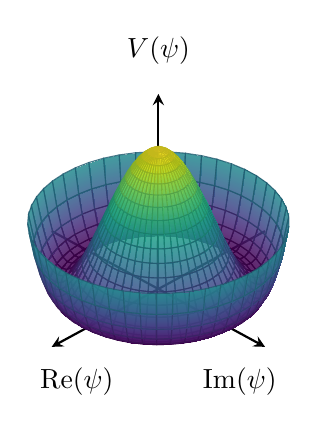
\begin{tikzpicture}
        \begin{axis}[
            view={135}{40}, 
            axis lines=center,
            axis line style={thick}, 
            axis on top=false,
            domain=0:360,
            y domain=0:1.3,      
            xmin=-1.5, xmax=1.5, 
            ymin=-1.5, ymax=1.5,
            zmin=0, zmax=1.4,    
            samples=50,
            samples y=25,
            xlabel=$\text{Re}(\psi)$,
            ylabel=$\text{Im}(\psi)$,
            zlabel=$V(\psi)$,
            xtick=\empty, ytick=\empty, ztick=\empty,
            colormap/viridis,
            % --- MODIFICHE ALLE ETICHETTE ---
            every axis x label/.style={at={(ticklabel* cs:1.10)}, anchor=north west},
            every axis y label/.style={at={(ticklabel* cs:1.10)}, anchor=north east},
            every axis z label/.style={at={(ticklabel* cs:1.10)}, anchor=south}, 
            % --------------------------------
            width=7cm, 
            height=7cm 
        ]
            % The potential surface
            \addplot3 [
                surf,
                shader=faceted interp,
                z buffer=sort,
                opacity=0.85 
            ] ({y*cos(x)}, {y*sin(x)}, {(y^2-1)^2});

        \end{axis}
    \end{tikzpicture}
    \caption{Ginzburg-Landau Theory: The Mexican-hat potential determining the equilibrium condensate density.}
    \label{fig:mexican_hat}
\end{figure}

For $T \ll T_c$, the large negative value of $\alpha$ sculpts the Mexican-hat potential into a very deep valley with a minimum at $\rho_0 = -\frac{\alpha}{\beta}$. In this deep mean-field approximation, creating spatial variations in the amplitude ($\nabla\sqrt{\rho} \neq 0$) requires a massive, prohibitive amount of energy to climb the steep walls of the potential well. Consequently, the amplitude ``freezes'' into a uniform, rigid density $\rho(\vec{r}) = \rho_0$, and $\nabla\sqrt{\rho} = 0$.

With the amplitude energetically locked at the bottom of the potential, the system can only host low-energy excitations by gently twisting the phase. The energy, therefore, simplifies strictly to the flow term:
\begin{equation}
    E(\theta) = E_0 + \int d^2\vec{r} \frac{\hbar^2\rho_0}{2m}(\nabla\theta)^2
\end{equation}
Ignoring the constant ground state energy $E_0$, we can explicitly define the superfluid stiffness (or helicity modulus) as:
\begin{equation}
    \rhos = \frac{\hbar^2\rho_0}{m}
\end{equation}
which yields exactly:
\begin{equation}
    E(\theta) = \frac{\rhos}{2} \int d^2\vec{r} (\nabla\theta)^2
\label{superconducting_energy}
\end{equation}

This final expression admits two profound and complementary physical interpretations \cite{chaikin1995principles}:
\begin{itemize}
    \item The Elastic Analogy (Stiffness): From a macroscopic thermodynamic perspective, this energy functional is mathematically analogous to the continuous theory of elasticity. Just as mechanically twisting a solid requires elastic strain energy proportional to the squared gradient of the displacement field, spatially twisting the quantum phase $\theta$ costs free energy. In this framework, $\rhos$ acts as the generalized elastic modulus (the stiffness) of the condensate, quantifying its rigidity against phase deformations.
    \item The Kinetic Interpretation: From a microscopic kinematic point of view, this term represents the macroscopic kinetic energy of the Cooper pairs. By defining the canonical superfluid velocity as $\mathbf{v}_s = \frac{\hbar}{m}\nabla\theta$, the energy density becomes exactly $\frac{1}{2}(m\rho_0)\mathbf{v}_s^2$, which matches the classical kinetic energy of a fluid with mass density $m\rho_0$ moving at velocity $\mathbf{v}_s$.
\end{itemize}

While this kinetic interpretation provides an intuitive picture, applying it to actual transport properties requires a more rigorous formulation. In quantum mechanics, the absolute macroscopic phase $\theta$ is not a directly measurable physical observable. Therefore, the theory must strictly respect gauge invariance: the measurable physical properties of the system must remain perfectly unchanged if we apply an arbitrary spatial shift to the phase, $\theta \to \theta + \chi(\vec{r})$. 

If the kinetic energy depended solely on the bare phase gradient $\nabla\theta$, such a mathematical shift would artificially alter the physical energy, fundamentally breaking the theory. To resolve this and obtain a physically meaningful velocity, we must couple the condensate to an electromagnetic field. Following the Ginzburg-Landau formalism, we introduce the magnetic vector potential $\mathbf{A}$ via the minimal coupling substitution. Because the vector potential possesses a corresponding gauge freedom ($\mathbf{A} \to \mathbf{A} + \frac{\hbar}{q}\nabla\chi$), it perfectly absorbs any arbitrary phase shift. The canonical phase gradient transforms as $\nabla\theta \to \nabla\theta - \frac{q}{\hbar}\mathbf{A}$, where $q = -2e$ is the charge of a Cooper pair. This substitution ensures that the true physical momentum remains gauge-invariant, yielding at $T=0$ the free energy:
\begin{equation}
    E(\theta, \mathbf{A}) = \frac{\rhos}{2} \int d^2\vec{r} \left( \nabla\theta - \frac{q}{\hbar}\mathbf{A} \right)^2
\end{equation}

Beyond ensuring theoretical consistency, embedding $\mathbf{A}$ into our equations provides the fundamental thermodynamic mechanism required to formally define the supercurrent. By temporarily keeping $\mathbf{A}$ in the framework, we can extract the macroscopic supercurrent density $\mathbf{J}$ using its rigorous thermodynamic definition as the variational derivative of the free energy (or energy at $T=0$) with respect to the vector potential: $\mathbf{J} = -\frac{\delta E}{\delta \mathbf{A}}$. Once this derivative is evaluated, we can isolate the behavior of pure external currents by turning off the external magnetic field ($\mathbf{A} = 0$), which yields:
\begin{equation}
    \mathbf{J} = \frac{q \rhos}{\hbar} \nabla\theta =\frac{q}{\hbar}\frac{\hbar^2\rho_0}{m}\nabla\theta= q \rho_0 \mathbf{v}_s
    \label{velocity}
\end{equation}
This confirms that in the absence of applied magnetic fields, the supercurrent is directly proportional to the spatial phase gradient, $\nabla\theta$, which drives the physical superfluid velocity.

This kinematic relationship naturally introduces the concept of a critical velocity, a central element of the computational models presented in this work. To drive a larger supercurrent through the material, the phase gradient must steepen, correspondingly increasing the local kinetic energy ($\frac{1}{2}mv_s^2$) of the flowing Cooper pairs. However, these pairs are bound together by a finite thermodynamic condensation energy. If the kinetic energy of the flow exceeds this binding energy, the pair is ripped apart. This physical threshold is known as the depairing critical velocity. Beyond this limit, the material locally loses its superconducting properties and transitions into a dissipative, normal state.

Finally, at equilibrium and well below the critical velocity, minimizing the unperturbed energy functional leads, as we shall see, directly to Laplace's equation, $\nabla^2\theta = 0$. This demonstrates that deep in the superconducting phase, the low-energy excitations and static current textures are entirely governed by the phase dynamics. By solving Laplace's equation with appropriate boundary conditions, we can map the physical current flow of the superconductor. As we will formally demonstrate, this macroscopic behavior is mathematically equivalent to the continuum limit of the classical XY model.

\section{The XY Model}
\subsection{From Lattice to Continuum}
While the Ginzburg-Landau theory provides a macroscopic description of the condensate, the XY model \cite{chaikin1995principles} serves as the fundamental starting point to study this phenomenology from a discrete lattice perspective. This model describes a system of classical spins confined to a plane, where each site $i$ of the lattice is characterized by an angle $\theta_i \in [0, 2\pi)$ representing the phase of the order parameter. 


Given the $O(2)$ rotational symmetry (or $U(1)$ symmetry in the context of superconductivity), the Hamiltonian on a lattice is defined as:
\begin{equation}
    H = -J \sum_{\langle i,j \rangle} \cos(\theta_i - \theta_j)
\end{equation}
where $J > 0$ is the ferromagnetic coupling constant, and the sum is extended over nearest neighbors. In this model, the minimum energy is achieved when all spins share the same angle.

To transition to the continuum limit, we first focus on the low-energy excitations of the system. In this regime, we assume that the phase variations between neighboring sites are extremely small, meaning $\Delta\theta_{ij} = \theta_i - \theta_j \ll 1$. We can therefore Taylor expand the cosine interaction:
\begin{equation}
    \cos(\Delta\theta_{ij}) \simeq 1 - \frac{1}{2}(\Delta\theta_{ij})^2 + \mathcal{O}(\Delta\theta_{ij}^4)
\end{equation}
Substituting this expansion into the Hamiltonian yields:
\begin{equation}
    H \simeq -J \sum_{\langle ij \rangle} 1 + \frac{J}{2} \sum_{\langle ij \rangle} (\theta_i - \theta_j)^2
\end{equation}
The first term evaluates to a massive negative constant representing the thermodynamic ground state energy. By ignoring this constant, which merely shifts the baseline energy scale, we obtain the effective low-energy quadratic Hamiltonian:
\begin{equation}
    H \simeq \frac{J}{2} \sum_{\langle i,j \rangle} (\theta_i - \theta_j)^2
\end{equation}

Next, we introduce a continuous, slowly varying macroscopic field $\theta(\vec{r})$ such that the phase at lattice site $i$ is exactly $\theta_i = \theta(\vec{r}_i)$. Assuming a two-dimensional square lattice with lattice parameter $a$, each site $i$ has nearest neighbors located at $\vec{r}_j = \vec{r}_i + \vec{a}$, where $\vec{a}$ represents the elementary lattice vectors with magnitude $|\vec{a}| = a$. To first order in $a$, the phase difference along a specific bond $\vec{a}$ is well approximated by the directional derivative:
\begin{equation}
    \theta_j - \theta_i = \theta(\vec{r}_i + \vec{a}) - \theta(\vec{r}_i) \simeq \vec{a} \cdot \nabla\theta(\vec{r}_i)
\end{equation}
To evaluate the sum over all nearest-neighbor pairs $\langle i,j \rangle$ without double-counting bonds, we rewrite it as a sum over every individual site $i$, restricting the bond vectors to only the two positive orthogonal directions: $\vec{a} \in \{a\hat{x}, a\hat{y}\}$. Squaring the phase differences for these two forward interactions gives the local continuous contribution:
\begin{equation}
    \sum_{\vec{a}} (\vec{a} \cdot \nabla\theta(\vec{r}_i))^2 = a^2(\partial_x\theta)^2 + a^2(\partial_y\theta)^2 = a^2|\nabla\theta(\vec{r}_i)|^2
\end{equation}
Substituting this local gradient back into the total energy, we obtain the discretized continuum Hamiltonian:
\begin{equation}
    H \approx \frac{J}{2} \sum_{i} a^2 |\nabla\theta(\vec{r}_i)|^2
\end{equation}

Finally, we take the formal continuum limit. In a 2D square lattice, each lattice site occupies an area of $a^2$. We can therefore transform the discrete sum over the sites into a spatial integral over the continuous plane, replacing the sum with $\int \frac{d^2\vec{r}}{a^2}$:
\begin{equation}
    H \simeq \frac{J}{2} \int \frac{d^2\vec{r}}{a^2} a^2 (\nabla\theta(\vec{r}))^2 = \frac{J}{2} \int d^2\vec{r} (\nabla\theta(\vec{r}))^2
\end{equation}

By formally identifying the microscopic coupling constant $J$ with the macroscopic superfluid stiffness $\rhos$, we exactly recover Eq.~\eqref{superconducting_energy} derived previously from the phenomenological Ginzburg-Landau theory:
\begin{equation}
    H[\theta(\vec{r})] = \frac{\rhos}{2} \int d^2\vec{r} (\nabla\theta(\vec{r}))^2
\end{equation}
This rigorous mathematical equivalence demonstrates that, deep in the superconducting state, the macroscopic behavior of the Cooper pair condensate is isomorphic to the continuum limit of the classical XY model.

\subsection{Equilibrium Condition}
We are now interested in finding the equilibrium condition. We calculate the functional derivative and set it to $0$:
\begin{equation}
    \frac{\delta H}{\delta\theta} = 0
\end{equation}
Let us consider a small perturbation $\epsilon\eta(\vec{r})$:
\begin{equation}
    H[\theta + \epsilon\eta] = \frac{\rhos}{2} \int d^2\vec{r} (\nabla(\theta + \epsilon\eta))^2 = \frac{\rhos}{2} \int d^2\vec{r} \left[ (\nabla\theta)^2 + 2\epsilon\nabla\theta \cdot \nabla\eta + \epsilon^2(\nabla\eta)^2 \right]
\end{equation}
To the first order in the perturbation $\epsilon$, the variation is:
\begin{equation}
    \delta H = \rhos \epsilon\int d^2\vec{r} \nabla\theta \cdot \nabla\eta
\end{equation}
Using the vector identity $\nabla\eta \cdot \nabla\theta=\nabla \cdot (\eta\nabla\theta)-\eta\nabla^2\theta$, we obtain:
\begin{equation}
    \delta H = \rhos\epsilon \int d^2\vec{r} \nabla \cdot (\eta\nabla\theta) - \rhos\epsilon \int d^2\vec{r} \eta\nabla^2\theta
\end{equation}
Assuming the field is fixed at the boundaries, meaning $\eta = 0$ on the Line $\partial A$, the divergence theorem gives:
\begin{equation}
    \int_A d^2r \nabla \cdot (\eta\nabla\theta) = \oint_{\partial A} dl \, \eta (\nabla\theta \cdot \hat{n}) = 0
\end{equation}
This leaves us with:
\begin{equation}
    \delta H = -\rhos\epsilon \int d^2\vec{r} \, \eta \nabla^2\theta
\end{equation}
Since this must hold for any arbitrary variation $\eta$, we obtain Laplace's equation:
\begin{equation}
    \nabla^2\theta(\vec{r}) = 0 \quad \implies \quad \frac{\partial^2\theta(\vec{r})}{\partial x^2} + \frac{\partial^2\theta(\vec{r})}{\partial y^2} = 0
\end{equation}
\section{Topological Configurations: Vortices}
The static phase field configurations that minimize the system's unperturbed energy must satisfy Laplace's equation, $\nabla^2 \theta = 0$. The most trivial solution to this equation is simply a uniform phase across the entire system ($\theta(\vec{r}) = \text{const.}$), which corresponds to the stationary ground state. However, alongside smooth, continuous phase variations, the system also admits non-trivial singular solutions known as vortices.

A vortex represents a topological defect in the order parameter. Because the macroscopic wave function must be single-valued, traversing any closed loop $\mathcal{C}$ around this singularity requires the phase $\theta$ to change by an integer multiple of $2\pi$:
\begin{equation}
    \oint_{\mathcal{C}} \nabla \theta \cdot d\mathbf{l} = 2\pi n, \quad n \in \mathbb{Z}
\end{equation}
where $n$ is the topological charge, or winding number. Assuming a symmetric circular flow, this circulation condition dictates that the phase gradient must decay inversely with the radial distance $r$ from the defect center:
\begin{equation}
    |\nabla \theta| = \frac{n}{r} \implies v_s(r) = \frac{\hbar n}{m r}
\end{equation}

This inverse relationship directly invokes the concept of critical velocity introduced previously. As one approaches the centreof the defect ($r \to 0$), the superfluid velocity $v_s$ diverges towards infinity. However, the physical supercurrent cannot exceed the depairing critical velocity. At a specific microscopic distance from the center, the local kinetic energy of the swirling Cooper pairs ($\frac{1}{2}mv_s^2$) exceeds their thermodynamic condensation energy. Consequently, the pairs break, and the amplitude of the order parameter collapses to zero ($\rho = 0$). 

This physical threshold defines the normal region: a non-superconducting, normal-state region at the centre of the vortex. The radius of this core $r_0$ is determined by the superconducting coherence length $\xi$ \cite{tinkham1996introduction}. The existence of this normal core is physically necessary to prevent the velocity, and thus the kinetic energy, from reaching unphysical infinite values at the origin.

Because the phase gradient represents the physical flow of the condensate, the energy of a single, isolated vortex is essentially the macroscopic kinetic energy of this circulating supercurrent. We obtain this energy by integrating the kinetic energy density over the area of the system. To avoid the unphysical divergence at the origin, we integrate from the boundary of the normal region $r_0$ out to the macroscopic system size $L$:
\begin{equation}
    E_{v} = \int_{r_0}^{L} \frac{1}{2} \rhos \left( \frac{n}{r} \right)^2 2\pi r dr = \pi \rhos n^2 \ln\left(\frac{L}{r_0}\right)
\end{equation}

This result reveals a profound topological consequence: the kinetic energy of an isolated vortex diverges logarithmically with the system size $L$. In the thermodynamic limit ($L \to \infty$), creating a single free vortex requires an infinite amount of energy, meaning that isolated vortices cannot spontaneously form at low temperatures.

\section{The Berezinskii-Kosterlitz-Thouless (BKT) Transition}

Although the present work focuses on the $T=0$ regime, understanding the Berezinskii-Kosterlitz-Thouless (BKT) transition is useful to contextualize current stability. According to the Mermin-Wagner theorem \cite{mermin1966absence}, long-range order cannot exist in 2D for $T>0$. However, Berezinskii \cite{berezinskii1971destruction, berezinskii1972destruction}, and subsequently Kosterlitz and Thouless \cite{kosterlitz1973ordering}, demonstrated that a topological phase transition related to vortex confinement does exist.

The free energy of a vortex is $F = E_v - TS$. Since the entropy associated with the vortex position is $S = k_B \ln(L/r_0)^2$, the free energy becomes:
\begin{equation}
    F = (\pi \rhos - 2k_B T) \ln\left(\frac{L}{r_0}\right)
\end{equation}
For $T < T_{BKT} = \frac{\pi \rhos}{2k_B}$, the energy dominates and vortices are forced to bind into neutral vortex-antivortex pairs ($n=+1, -1$). In this regime, the system exhibits quasi-long-range order with algebraic decay of correlations. Above $T_{BKT}$, the pairs dissociate (unbinding) into a gas of free vortices, destroying superconductivity.

\section{Analysis in the Zero-Temperature Limit}

In the specific framework developed in this thesis, we operate strictly in the zero-temperature limit ($T=0$). In this regime:
\begin{enumerate}
    \item Thermal fluctuations are entirely suppressed; consequently, the thermally driven BKT transition does not occur, meaning vortex-antivortex pairs neither spontaneously nucleate nor thermally dissociate.
    \item The system resides in a state of maximum phase coherence, where the superfluid stiffness $\rho_s$ assumes its unrenormalized, bare value.
    \item The presence of topological defects is dictated exclusively by external constraints (such as localized pinning centers) or rigidly imposed boundary conditions (fixed topological winding numbers).
\end{enumerate}

In this static regime, the theoretical problem reduces to finding the macroscopic phase field configuration that minimizes the kinetic energy of the condensate within confined geometries---a task for which the mathematical formalism of complex potential flow and conformal mapping is exceptionally well-suited. 

Throughout the following analysis, we assume that the spatial coordinates of the vortices are rigidly fixed by external pinning forces. While the precise physical mechanism responsible for establishing these initially pinned configurations falls outside the scope of this dissertation, it is physically well-founded to consider that local magnetic interactions, such as those provided by surface-deposited nanomagnets, can stably anchor vortices of arbitrary polarity \cite{martin1997artificial}. For the sake of analytical clarity, we also assume that the local vector potential generated by these external pinning centers can be neglected in the following analysis.

Consequently, our investigation strictly focuses on the response of this established ground state to uniform external transport currents, with a particular emphasis on the resulting non-linear deformations of the normal core boundaries.

% ==========================================
% CHAPTER 2: CONFORMAL MAPPING AND COMPLEX POTENTIAL
% ==========================================
\chapter{Mathematical Methods: Conformal Mapping}

\section{Mathematical Foundations}
\label{mathmetods}
The problem of determining superconducting currents in a two-dimensional system reduces to solving Laplace's equation for the phase field. Outside the normal regions, the phase field $\theta(x,y)$ satisfies:
\begin{equation}
    \nabla^2 \theta(x,y) = 0
\end{equation}
In two dimensions, there is a profound connection between the solutions of Laplace's equation (harmonic functions) and analytic functions of a complex variable $z = x + iy$. A complex function $f(z) = u(x,y) + iv(x,y)$ is analytic if it satisfies the Cauchy-Riemann conditions:
\begin{equation}
    \frac{\partial u}{\partial x} = \frac{\partial v}{\partial y}, \quad \frac{\partial u}{\partial y} = -\frac{\partial v}{\partial x}
\end{equation}
These conditions immediately imply that both the real and imaginary parts of $f(z)$ are harmonic. To demonstrate this explicitly, we assume that the function is analytic, meaning its real and imaginary components have continuous second partial derivatives. According to Schwarz's theorem, the mixed second-order partial derivatives are symmetric:
\begin{equation}
    \frac{\partial^2}{\partial x \partial y} = \frac{\partial^2}{\partial y \partial x}
\end{equation}

To prove that $u(x,y)$ is harmonic, we differentiate the first Cauchy-Riemann condition with respect to $x$, and the second with respect to $y$:
\begin{equation}
    \frac{\partial^2 u}{\partial x^2} = \frac{\partial^2 v}{\partial x \partial y}, \quad \frac{\partial^2 u}{\partial y^2} = -\frac{\partial^2 v}{\partial y \partial x}
\end{equation}
Summing these two equations yields the Laplacian of $u$:
\begin{equation}
    \nabla^2 u = \frac{\partial^2 u}{\partial x^2} + \frac{\partial^2 u}{\partial y^2} = \frac{\partial^2 v}{\partial x \partial y} - \frac{\partial^2 v}{\partial y \partial x} = 0
\end{equation}
Thus, $u(x,y)$ satisfies Laplace's equation. 

An identical procedure can be applied to the imaginary part, $v(x,y)$. By differentiating the first Cauchy-Riemann condition with respect to $y$, and the second with respect to $x$, we obtain:
\begin{equation}
    \frac{\partial^2 v}{\partial y^2} = \frac{\partial^2 u}{\partial y \partial x}, \quad -\frac{\partial^2 v}{\partial x^2} = \frac{\partial^2 u}{\partial x \partial y}
\end{equation}
Subtracting the second equation from the first gives the Laplacian of $v$:
\begin{equation}
    \nabla^2 v = \frac{\partial^2 v}{\partial x^2} + \frac{\partial^2 v}{\partial y^2} = -\frac{\partial^2 u}{\partial x \partial y} + \frac{\partial^2 u}{\partial y \partial x} = 0
\end{equation}
proving that $v(x,y)$ is also a harmonic function \cite{brown2013complex}. 

This duality allows us to treat the macroscopic phase field of the superconductor as either the real or imaginary part of an analytic complex potential, opening the door to the powerful technique of conformal mapping \cite{clem2011geometry}.

\section{The Complex Potential for Superfluids}
We define the dimensionless complex potential $f(z)$ as \cite{kogan2014manipulating}:
\begin{equation}
    f(z) = \psi(x,y) + i\theta(x,y)
\end{equation}
where:
\begin{itemize}
    \item $\psi(x,y)$ is the stream function (note that here $\psi$ does not denote the Ginzburg-Landau order parameter amplitude introduced in~\ref{cap:physicsframework}). The lines $\psi(x,y) = \text{constant}$ represent the physical trajectories followed by the superconducting currents (the streamlines).
    \item $\theta(x,y)$ is the scalar potential representing the macroscopic quantum phase of the condensate.
\end{itemize}

It is strictly necessary to clarify the dimensional units of this formulation.  We can consider lengths defined so far in units of the core radius, $r_0$.  Then, since the phase $\theta$ is inherently dimensionless; the physical gradient is $\frac{1}{r_0}\nabla $, where $\nabla$ is dimensionless, and the physical superfluid velocity $\mathbf{v}_s$ is:
\begin{equation}
    \mathbf{v}_s = \frac{\hbar}{m r_0} \nabla \theta
\end{equation}

To make the complex potential mathematically consistent with classical fluid dynamics---where a velocity potential has kinematic dimensions of $[L]^2[T]^{-1}$---we can define the physical complex potential $F(z)$ as:
\begin{equation}
    F(z) = \frac{\hbar}{m} f(z) = \frac{\hbar}{m} \psi(x,y) + i \frac{\hbar}{m} \theta(x,y)
\end{equation}
In this physical gauge, the scaled phase $\Phi = \frac{\hbar}{m}\theta$ acts as the true velocity potential ($\mathbf{v}_s = \nabla \Phi$), and the scaled stream function $\Psi = \frac{\hbar}{m}\psi$ dictates the physical volumetric flow rate between streamlines. 
In the following we work in units such that $\frac{\hbar}{m}=1$ and restore units when convenient for clarity. In this formalism, the current density is given by Eq.~\eqref{velocity} and Laplace's equation is equivalent to the condition of current conservation:
$$
\nabla \cdot \mathbf{J} = q\rho_0\frac{\hbar}{mr^2_0}\nabla^2\theta = 0
$$

The conformal approach is highly powerful because any analytic transformation $w = g(z)$ strictly preserves the Cauchy-Riemann conditions, and therefore preserves the structure of Laplace's equation. If we know the solution for $f(z)$ in a simple domain (e.g., the infinite plane), we can map this solution into a geometrically complex domain while completely maintaining the physical validity of the flow lines and the phase field.

\subsection{The Complex Velocity}
The usefulness of the complex potential lies in the ease with which the superfluid velocity field can be extracted. By differentiating $f(z)$ with respect to the complex variable $z$, we obtain the so-called complex velocity $W(z)$. Using the Cauchy-Riemann conditions, we have:
\begin{equation}
    W(z) = \frac{df}{dz} = \frac{\partial \psi}{\partial x} + i \frac{\partial \theta}{\partial x}
\end{equation}
Since the physical velocity is related to the phase gradient, $\mathbf{v} \propto \nabla \theta = (\partial_x \theta, \partial_y \theta)$, and by the Cauchy-Riemann equations $\partial_x \psi = \partial_y \theta = v_y$, we can write:
\begin{equation}
    v_x - i v_y = -i \frac{df}{dz}
\end{equation}
A direct and highly useful consequence of this formulation is that the square modulus of the physical fluid velocity is exactly equal to the square modulus of the complex velocity:
\begin{equation}
    |\mathbf{v}|^2 = v_x^2 + v_y^2 = |W(z)|^2 = \left| \frac{df}{dz} \right|^2
\end{equation}
This property is particularly advantageous, as it allows for the kinetic energy density of the superfluid to be computed directly from the complex derivative. Overall, this operator directly and algebraically maps the complex topology of the currents into a differentiable analytic function.

\section{Fundamental Solutions}
Based on the analogy with electrostatics and fluid dynamics, we can identify the analytic functions corresponding to the configurations of interest in the superconductor:

\begin{enumerate}
    \item Isolated Vortex: A vortex with a unit topological charge positioned at the origin is described by the potential:
    \begin{equation}
        f(z) = \log(z) = \ln(r) + i\theta
    \end{equation}
    Here, the imaginary part (the phase) coincides with the azimuthal angle $\phi$, i.e. $\phi=\theta $. Then the phase satisfies the circulation condition $\oint \nabla \theta \cdot d\mathbf{l} = 2\pi$. In the following, we fix the units of length such that $r_0=1$. Implicitly, this also defines the critical velocity of our superconductor: indeed, we can define the unit of critical velocity by calculating the intrinsic superfluid velocity at the boundary $r_0=1$ in the absence of an external current. 
    Differentiating the potential with respect to $z$ yields the complex velocity field:
    $$W(z)=f'(z) = \frac{1}{z}$$
    Evaluating the magnitude of this intrinsic velocity precisely at the boundary of the core ($z = e^{i\theta}$) defines our critical velocity:        
    \begin{equation}
    v_c=|W(e^{i\theta})| = \left| f'(e^{i\theta}) \right| = \left| e^{-i\theta} \right| = 1
    \label{criticalvelocity}
    \end{equation}
    This demonstrates that in our dimensionless unit system, the maximum supercurrent that the defect naturally sustains at its edge serves as the units of velocity. 
    Restoring units, we have $v_c=\frac{\hbar}{r_0m}$ and $\mathbf{v}=v_c \nabla \theta$, where the gradient is dimensionless.
    
    \begin{figure}[H]
        \centering
        \begin{subfigure}[t]{0.48\textwidth}
            \centering
            
\includegraphics[width=\linewidth,height=5.2cm,keepaspectratio]{Grafici/Grafici_Particolari/1_FlussoPotenziale_onlyvortex_c0.1.pdf}
            \caption{Streamlines and isolines. The difference in phase between two isolines of $\theta(\mathbf{r})$ is $\Delta\theta=\frac{\pi}{6}=30^\circ$; the absence of the $0/2\pi n$ isoline on the left side of the figure is due to the presence of a branch cut.}
            \label{fig:vortex_streamlines}
        \end{subfigure}
        \hfill
        \begin{subfigure}[t]{0.48\textwidth}
            \centering
             
\includegraphics[width=\linewidth,height=5.2cm,keepaspectratio]{Grafici/Grafici_Particolari/3_Gradiente_onlyvortex_c0.1.pdf}
            \caption{Velocity field.}
            \label{fig:vortex_velocity}
        \end{subfigure}
        \caption{Isolated Vortex ($j_0=0$): Visualization of the complex potential $f(z) = \log(z)$ and the associated velocity field. The white region at the center is the normal state core which, in our units, has radius $r_0=1$.}
        \label{fig:isolated_onlyvortex}
    \end{figure}

\item Circular defect in a Uniform Flow: By leveraging the principle of linear superposition and the Milne-Thomson circle theorem \cite{milne1968theoretical}, we can model circular defects made of an insulator or a normal metal. If we apply an external current, we can impose that far from the region of the defect the current is uniform and coincides with the external current. This can be represented by $f_\text{ext}=ij_0z$, which, restoring the units, corresponds to a current density $\mathbf{J}_\text{ext}=q\rho_0\frac{\hbar}{mr_0}j_0$. The function representing the current around the defect of radius $r_0=1$ reads:
    \begin{equation}
        f(z) = ij_0 \left(z + \frac{1}{z}\right)
        \label{emptygeometry}
    \end{equation}
    It is easy to check that the real part of this potential (the stream function $\psi$) is exactly zero at $|z| = 1$. This mathematically enforces the physical boundary condition that superconducting Cooper pairs cannot flow into the normal region, as shown in Fig.~\ref{fig:empty_hole}.

    \begin{figure}[H]
        \centering
        \begin{subfigure}[t]{0.48\textwidth}
            \centering
            
\includegraphics[width=\linewidth,height=5.2cm,keepaspectratio]{Grafici/Grafici_Particolari/1_FlussoPotenziale_onlyhole_c0.1.pdf}
            \caption{Streamlines and isolines.}
            \label{fig:hole_streamlines}
        \end{subfigure}
        \hfill
        \begin{subfigure}[t]{0.48\textwidth}
            \centering
             
\includegraphics[width=\linewidth,height=5.2cm,keepaspectratio]{Grafici/Grafici_Particolari/3_Gradiente_onlyhole_c0.1.pdf}
            \caption{Velocity field.}
            \label{fig:hole_velocity}
        \end{subfigure}
        \caption{Circular Defect in Uniform Flow ($j_0=0.1$): Superfluid flow deflecting around an insulating (normal) circular defect of radius 1, demonstrating the vanishing perpendicular velocity at the boundary.}
        \label{fig:empty_hole}
    \end{figure}
\end{enumerate}
  
% ==========================================
% CHAPTER 3: COMPUTATIONAL ANALYSIS
% ==========================================
% CHAPTER 3: SINGLE VORTEX CONFIGURATION
% ==========================================
\chapter{Single Vortex Configuration}
\label{cap:single_vortex}

In this chapter, we investigate the behavior of an isolated vortex trapped in a two-dimensional superconductor driven by a uniform external current. Throughout this text, we define the vortex as a fixed topological singularity with a normal region representing the vortex core. The geometry of this non-superconducting domain is governed by two fundamental boundary conditions. First, its physical boundary perfectly aligns with the critical velocity threshold, $|\mathbf{v}|=1$, consistently with Eq.~\eqref{criticalvelocity}. Second, the normal core acts as an impenetrable obstacle, meaning no supercurrent can penetrate inside the critical line ($\mathbf{J}_{\perp}=0$): this impenetrability captures the physical fact that current will naturally bypass a region of finite resistance to flow exclusively through the surrounding zero-resistance superconducting phase. 
We will see that the external current deforms the shape of the core and our purpose will be to take into account this effect.
We first formulate the $0^{\text{th}}$ order baseline model with a rigid normal region, then introduce a $1^{\text{st}}$ order geometric feedback model to account for core deformation, and finally present and analyze the resulting numerical solutions and velocity fields across various external current regimes.

\section{Zeroth-Order Approximation}
\label{sec:zeroordervortex}
To study this phenomenon, we first define the zeroth-order approximation of our system. In this unperturbed baseline model, we assume the physical boundary of the normal region and the topological singularity (the vortex) perfectly coincide and remain completely rigid under the application of an external current. We assume the vortex is strongly pinned and immobile; the specific microscopic pinning mechanisms (e.g., magnetic dots) fall outside the scope of this dissertation.  
    
To describe a vortex with a rigid circular normal region in the presence of an external current, we add a vortex term to Eq.~\eqref{emptygeometry} describing a uniform current with a circular defect. Under our dimensionless units, the complete zeroth-order potential is:
\begin{equation}
    f(z) = ij_0 \left(z + \frac{1}{z}\right) + \log(z)
\label{singledefect}
\end{equation}
As we shall see, this expression geometrically captures the asymmetric current flow around a rigid normal region without carrying explicit physical constants.

\begin{figure}[H]
    \centering
    \begin{subfigure}[t]{0.48\textwidth}
        \centering
        
\includegraphics[width=\linewidth,height=5.2cm,keepaspectratio]{Grafici/Grafici_Particolari/1_FlussoPotenziale_complete_c0.1.pdf}
        \caption{Streamlines and isolines. The difference in phase between two isolines of $\theta(\mathbf{r})$ is $\Delta\theta=\frac{\pi}{6}=30^\circ$.}
        \label{fig:fixed_streamlines}
    \end{subfigure}
    \hfill
    \begin{subfigure}[t]{0.48\textwidth}
        \centering
         
\includegraphics[width=\linewidth,height=5.2cm,keepaspectratio]{Grafici/Grafici_Particolari/3_Gradiente_complete_c0.1.pdf}
        \caption{Velocity field.}
        \label{fig:fixed_velocity}
    
    \end{subfigure}
    \caption{Fixed Vortex with Rigid Normal Region ($j_0=0.1$): Asymmetric current flow resulting from the superposition of an external uniform external current ($j_0=0.1$) and a trapped topological vortex with a circular normal region at the center whose boundary is represented by the black full line. The dashed blue line represents the critical isoline $|\mathbf{v}|=1$.}
    \label{fig:fixed_onlyvortex}
\end{figure}

As expected from the presence of a vortex term, Fig.~\ref{fig:fixed_onlyvortex} shows that the superposition of the external current and the circulating vortex current creates an asymmetry in the total velocity field. As a consequence, the currents add constructively on one side of the vortex (the lower part of the figure) and destructively on the other. To understand the physical implications of this asymmetry, we examine the behavior of the system under different external currents:
\begin{itemize}
    \item Unperturbed System: Without an external current ($j_0=0$), the isoline corresponding to the critical velocity threshold ($|\mathbf{v}| = 1$) perfectly coincides with the geometric boundary of the normal region, described by the unit circle centered at the origin.
    \item Addition of External Current: Upon introducing the external current ($j_0 \neq 0$), the constructive superposition causes the local current magnitude to exceed the critical limit. The velocity field deforms and the isoline $|\mathbf{v}| = 1$ changes, no longer matching the normal region (Fig.~\ref{fig:fixed_onlyvortex}), that is to say the region where the impenetrable condition was initially imposed. Notice that the superconducting solution can be analytically continued into the nominally normal region, i.e., inside the unit circle. Here and in the plots below, the dashed blue line inside the white region corresponds to that solution.  In the following, we will refer to the $|\mathbf{v}|=1$ line as the $0^{\text{th}}$ order critical line or isoline. 
\end{itemize}
 

To characterize the current-driven deformation we computed the intersections of the critical line with the $y$-axis, identifying the extremal coordinates $y_{\text{min}}$ and $y_{\text{max}}$. Fig.~\ref{fig:results_pre_coords} illustrates the extremal coordinates of the $0^{\text{th}}$ order system.

\begin{figure}[H]
    \centering
    \begin{subfigure}[t]{0.48\textwidth}
        \centering
        
\includegraphics[width=\linewidth,height=5.2cm,keepaspectratio]{Grafici/Grafici_Generici/maxminY_pre_coords.pdf}
        \caption{$0^{\text{th}}$ Order extremal vertical coordinates.}
        \label{fig:maxminY_pre}
    \end{subfigure}
    \hfill
    \begin{subfigure}[t]{0.48\textwidth}
        \centering
         
\includegraphics[width=\linewidth,height=5.2cm,keepaspectratio]{Grafici/Grafici_Generici/maxminX_traslato_pre_coords.pdf}
        \caption{$0^{\text{th}}$ Order extremal horizontal coordinates.}
        \label{fig:maxminX_pre}
    \end{subfigure}
    \caption{Single Vortex ($0^{\text{th}}$ Order): Variation of the extremal coordinates comparing the normal region (continuous lines) to the critical isoline (dashed lines) in the $0^{\text{th}}$ Order Model.}
    \label{fig:results_pre_coords}
\end{figure}

By decoupling the boundary into vertical and horizontal components, the data explicitly reveals the anisotropy of the perturbation: as the magnitude of the external current $|j_0|$ increases, the critical isoline undergoes severe spatial stretching along the $y$-axis (Fig.~\ref{fig:maxminY_pre}), while its horizontal width calculated on the axis containing the center of the normal region (the $x$-axis, in this case) remains relatively rigid (Fig.~\ref{fig:maxminX_pre}). This demonstrates that the physical boundary is not merely translating, but actively deforming. Furthermore, as expected, we see that as $|j_0|$ increases, the alignment between the critical isoline and the normal region gets worse. The kink of the full lines at $j_0\approx\pm0.2$ will become clear later.

This misalignment makes the model non-self-consistent. To find a self-consistent solution where the critical line and the boundary of the normal region coincide is beyond the present scope. Instead we present a strategy to mitigate the problem. We achieve this by introducing a first-order approximation driven by a spatial feedback mechanism. The constructive superposition of the external current and the vortex circulation breaks spatial symmetry, amplifying the local velocity southward ($y < 0$) while suppressing it northward ($y > 0$). Consequently, introducing a vertical spatial shift ($d < 0$) to the normal region improves the alignment between its perimeter and the deformed critical isoline, while the topological singularity remains firmly anchored at the origin. By symmetry, an identical but geometrically mirrored analysis applies for a negative external current ($j_0 < 0$), where the deformation and the corresponding spatial correction are simply reflected across the horizontal axis.

\section{First-Order Approximation}
\label{sec:sv_first}
In order to mitigate the non-self-consistency identified in the $0^{\text{th}}$ order model, this section analyzes the system's geometric response using a first-order approximation. We expect that for small $|j_0|$ the critical line remains approximately circular and simply displaces by an amount $d$ along the $y$ direction, without deforming. The challenge, then, is to displace the boundary of the normal region so that it coincides with its own critical line, while the topological vortex center remains fixed. To achieve the alignment between the normal region and the critical line, several feedback criteria were evaluated. 

We start by computing analytically the  extremal coordinates of the $0^{\text{th}}$ order critical line shown in Fig.~\ref{fig:results_pre_coords}. The velocity field is obtained by taking the complex derivative of the original potential $f(z)$ (see Chapter~\ref{mathmetods}):
\begin{equation}
    W(z) = f'(z) = ij_0 \left( 1 - \frac{1}{z^2} \right) + \frac{1}{z}
\end{equation}
Since we are interested in the intersection of the critical line with the imaginary axis, we evaluate this expression at $z=iy$:
\begin{equation}
    W(iy) = ij_0 \left( 1 + \frac{1}{y^2} \right) - i \frac{1}{y} = i \left( \frac{j_0 y^2 - y + j_0}{y^2} \right)
\end{equation}

Imposing the critical isoline condition $|W(iy)|^2=1$, we obtain:
\begin{equation}
    \left( \frac{j_0 y^2 - y + j_0}{y^2} \right)^2 = 1 \implies (j_0 y^2 - y + j_0)^2 = y^4
\end{equation}

Instead of squaring the trinomial and proceeding with implicit differentiation, we can recognize that the expression $(j_0 y^2 - y + j_0)^2 - y^4 = 0$ is a difference of squares. Grouping the terms yields the product of two independent quadratic factors:
\begin{equation}
    [(j_0 - 1)y^2 - y + j_0] \cdot [(j_0+1)y^2 - y + j_0] = 0
    \label{solutions}
\end{equation}

To accurately map the vertical spatial extension of the critical lobes along the symmetry axis, we must evaluate all four possible analytic solutions arising from these two factors. The number of real, physical roots depends strictly on the applied current $j_0$ and the non-negativity of the respective discriminants:
\begin{itemize}
    \item The first factor yields real roots when $j_0 \in \left[\frac{1 - \sqrt{2}}{2}, \frac{1 + \sqrt{2}}{2}\right]$ (approximately $-0.207 \le j_0 \le 1.207$).
    \item The second factor yields real roots when $j_0 \in \left[\frac{-1 - \sqrt{2}}{2}, \frac{-1 + \sqrt{2}}{2}\right]$ (approximately $-1.207 \le j_0 \le 0.207$).
\end{itemize}
However, it is important to note that these mathematical intervals extend beyond the physical regime of the system. The magnitude of the external current is fundamentally bounded by the inequality $|j_0| \le 1$, which represents the critical current far from the defect. Since the critical velocity in our dimensionless units is defined as $|\mathbf{v}|=1$, any asymptotic current exceeding this threshold ($|j_0| \ge 1$) would induce a global transition to the dissipative normal state, rendering the defect model physically irrelevant. Within this physically permissible range, the system exhibits distinct algebraic regimes characterized by the number of valid roots. For small currents lying within the overlap interval $j_0 \in \left[\frac{1 - \sqrt{2}}{2}, \frac{-1 + \sqrt{2}}{2}\right]$, both discriminants are non-negative, and the governing equation produces exactly four real solutions. Outside of this specific region, one of the quadratic factors evaluates to complex roots and can be discarded, leaving only two real solutions. This explains the kink shown in Fig.~\ref{fig:results_pre_coords}.
To determine the physical boundaries of the critical line, we compute all available real roots for a given $j_0$: we define the smallest real root as $y_{\text{min}}$ and the largest real root as $y_{\text{max}}$. 

We then tested three different geometric corrections in order to determine the optimized normal region trying to follow the deformation of the critical line:
\begin{enumerate}
    \item $d = \frac{y_{\text{max}} + y_{\text{min}}}{2}$: This correction places the center of the optimized normal region exactly in the middle of the $0^{\text{th}}$ order critical line.
    \item $d = \frac{y_{\text{max}} + y_{\text{min}}}{4}$: This correction places the optimized normal region at the midpoint between the original normal region (centered at the origin, in this case) and the center of the $0^{\text{th}}$ order critical line.
    \item $d = y_{\text{min}} + 1$ (for $j_0 \ge 0$) or $d = y_{\text{max}} - 1$ (for $j_0 < 0$): Given the unit radius ($r_0=1$), this correction aligns the lower edge of the normal region precisely with the minimum extremum of the $0^{\text{th}}$ order critical line when $j_0 \ge 0$, and aligns the upper edge with the maximum extremum when $j_0 < 0$, ensuring physical symmetry under current reversal.
\end{enumerate}
We will refer to these approximations as the 1/2 Feedback Model, the 1/4 Feedback Model and the Extremal Feedback Model, respectively. Incorporating this spatial shift, the updated complex potential becomes:
\begin{equation}
    f_{\text{new}}(z) = ij_0 \left( z + \frac{1}{z-d} \right) + \log(z)
\end{equation}
Notice once again a fundamental physical distinction in this corrected potential: while the circular boundary is shifted by a distance $d$, the vortex (represented by the logarithmic term) remains firmly anchored at its original position.

As we have previously done in Sec. \ref{sec:zeroordervortex}, to rigorously quantify the geometric agreement between the new $1^{\text{st}}$ Order normal region and critical line and verify whether our feedback model successfully approximates a self-consistent solution, in Fig. \ref{fig:results_post_coords} we evaluate the extremal coordinate deviations. 

\begin{figure}[H]
    \centering
    \begin{subfigure}[t]{0.48\textwidth}
        \centering
         
\includegraphics[width=\linewidth,height=5.2cm,keepaspectratio]{Grafici/Grafici_Generici/maxminY_post_coords.pdf}
        \caption{$1^{\text{st}}$ Order extremal vertical coordinates.}
        \label{fig:maxminY_post}
    \end{subfigure}
    \hfill
    \begin{subfigure}[t]{0.48\textwidth}
        \centering
         
\includegraphics[width=\linewidth,height=5.2cm,keepaspectratio]{Grafici/Grafici_Generici/maxminX_traslato_post_coords.pdf}
        \caption{$1^{\text{st}}$ Order extremal horizontal coordinates.}
        \label{fig:maxminX_post}
    \end{subfigure}
    \caption{Single Vortex ($1^{\text{st}}$ Order): Variation of the extremal coordinates comparing the normal region (continuous lines) to the critical isoline (dashed lines) in the $1^{\text{st}}$ Order Model.}
    \label{fig:results_post_coords}
\end{figure}

These $1^{\text{st}}$ order extremal coordinates serve to validate the different approximations. In general, the vertical data (Fig. \ref{fig:maxminY_post}) confirms that shifting the core successfully reduces the dominant spatial discrepancy; this is visually confirmed by observing that the boundaries representing the normal region and the critical isoline are significantly closer than in the $0^{\text{th}}$ order baseline.. However, this decoupled analysis simultaneously exposes the inherent geometric trade-off of applying a translation to a more complex deformed line: optimizing the vertical alignment inevitably introduces slight boundary mismatches along the horizontal axis (Fig. \ref{fig:maxminX_post}). 

From this systematic comparison, several key observations emerge:
\begin{itemize}
    \item Invariance to Correction Type: The specific method of geometric correction does not significantly influence the overall qualitative behavior. No single approximation drastically outperforms the others across the entire parameter space. However, we will see in Sec. \ref{sec:particularconfig} that locally, in specific regimes of the external current, there could be differences in their performance.
    \item Validity Regime and Asymptotic Convergence: All correction methods perform remarkably well in the low-current regime ($|j_0| < 0.2$), where horizontal discrepancies remain entirely marginal. As the external current approaches zero ($j_0 \to 0$), the spatial discrepancy between the boundary of the normal region and the critical line vanishes. This behavior is perfectly consistent with the mathematical premise that our first-order approximation is mainly valid for small values of the external current (Sec.~\ref{sec:sv_first}). Furthermore, this strong low-current convergence suggests that a continuous, iterative application of this geometric feedback loop might yield a self-consistent solution for the boundaries of the superconducting state.
    \item Current Reversal Symmetry: The configuration is invariant under the transformation $j_0 \to -j_0$ combined with spatial inversion $y\rightarrow-y$. Specifically, under current reversal, the local velocity profile and the resulting normal domain deformation mirror across the horizontal axis. Consequently, the critical external current magnitude required to induce a new shape of the normal region is identical in both directions ($|j_{0,+}| = |j_{0,-}|$), demonstrating that the isolated single vortex configuration remains strictly reciprocal in terms of macroscopic transport properties. While the localization of the normal deformation shifts between upper and lower defect boundaries depending on current sign, true macroscopic non-reciprocity, as we shall see in Chapter~\ref{cap:dipolar_configuration}, emerges only in dipolar configurations where multi-defect interference breaks reversal symmetry globally.
    \item Critical Value: A marked transition in the system's geometric behavior occurs near $|j_0|\approx0.2$. This threshold corresponds directly to the change in the number of real roots of Eq.~\eqref{solutions}. We will discuss this transition in further detail later in Sec. \ref{sec:medium_current}.
\end{itemize}
\subsection{Particular Current Values for the Single Vortex Configuration}
\label{sec:particularconfig}
This section demonstrates how the geometric feedback method operates under specific configurations. Specifically, we investigate the spatial and topological adjustments required to stabilize the superconducting phase boundaries across three distinct regimes: weak, medium, and high external currents. Because the system is reciprocal, we present results only for positive values of $j_0$; for negative values of the external current, identical deformations and flow topologies are obtained, simply mirrored across the horizontal axis.

\subsubsection{Weak Current $j_0=0.1$}
In this subsection, we present a detailed analysis of the flow topology and velocity fields for a specific low-current regime ($j_0=0.1$). The various geometric feedback models exhibit highly accurate behavior in this regime. To observe the macroscopic flow, Fig.~\ref{fig:feedback_flusso} illustrates the complex potential streamlines and phase isolines for the unperturbed baseline compared to the three $1^{\text{st}}$ order corrections.

% =========================================================
% FIGURA 1: FLUSSO E POTENZIALE
% =========================================================
\begin{figure}[H]
    \centering
    \begin{subfigure}[t]{0.48\textwidth}
        \centering
        
\includegraphics[width=\linewidth,height=5.2cm,keepaspectratio]{Grafici/Grafici_Particolari/1_FlussoPotenziale_nocorr_c0.1.pdf}
        \caption{$0^{\text{th}}$ Order Model}
        \label{fig:flusso_nocorr}
    \end{subfigure}
    \hfill
    \begin{subfigure}[t]{0.48\textwidth}
        \centering
        
\includegraphics[width=\linewidth,height=5.2cm,keepaspectratio]{Grafici/Grafici_Particolari/1_FlussoPotenziale_corr_noappr_c0.1.pdf}
        \caption{1/2 Feedback Model}
        \label{fig:flusso_corr_noappr}
    \end{subfigure}
    
    \vspace{0.4cm}
    
    \begin{subfigure}[t]{0.48\textwidth}
        \centering
        
\includegraphics[width=\linewidth,height=5.2cm,keepaspectratio]{Grafici/Grafici_Particolari/1_FlussoPotenziale_corr_mean_c0.1.pdf}
        \caption{1/4 Feedback Model}
        \label{fig:flusso_corr_mean}
    \end{subfigure}
    \hfill
    \begin{subfigure}[t]{0.48\textwidth}
        \centering
        
\includegraphics[width=\linewidth,height=5.2cm,keepaspectratio]{Grafici/Grafici_Particolari/1_FlussoPotenziale_corr_min_c0.1.pdf}
        \caption{Extremal Feedback Model}
        \label{fig:flusso_corr_min}
    \end{subfigure}
    \caption{Single Vortex ($j_0=0.1$): Comparison of the complex potential streamlines and isolines around the defect for all four models in the low current regime. The difference in phase between two isolines of $\theta(\mathbf{r})$ is $\Delta\theta=\frac{\pi}{6}=30^\circ$.}
    \label{fig:feedback_flusso}
\end{figure}

To visualize the local flow variations and the directionality of the supercurrent around the dissipative normal phase regions, we examine the gradient vector fields in Fig.~\ref{fig:feedback_gradient}, which explicitly map the local velocity vectors across the different models.

% =========================================================
% FIGURA 2: GRADIENTE CON FRECCE
% =========================================================
\begin{figure}[H]
    \centering
    \begin{subfigure}[t]{0.48\textwidth}
        \centering
        
\includegraphics[width=\linewidth,height=5.2cm,keepaspectratio]{Grafici/Grafici_Particolari/3_Gradiente_nocorr_c0.1.pdf}
        \caption{$0^{\text{th}}$ Order Model}
        \label{fig:grad_nocorr}
    \end{subfigure}
    \hfill
    \begin{subfigure}[t]{0.48\textwidth}
        \centering
        
\includegraphics[width=\linewidth,height=5.2cm,keepaspectratio]{Grafici/Grafici_Particolari/3_Gradiente_corr_noappr_c0.1.pdf}
        \caption{1/2 Feedback Model}
        \label{fig:grad_corr_noappr}
    \end{subfigure}
    
    \vspace{0.4cm}
    
    \begin{subfigure}[t]{0.48\textwidth}
        \centering
        
\includegraphics[width=\linewidth,height=5.2cm,keepaspectratio]{Grafici/Grafici_Particolari/3_Gradiente_corr_mean_c0.1.pdf}
        \caption{1/4 Feedback Model}
        \label{fig:grad_corr_mean}
    \end{subfigure}
    \hfill
    \begin{subfigure}[t]{0.48\textwidth}
        \centering
        
\includegraphics[width=\linewidth,height=5.2cm,keepaspectratio]{Grafici/Grafici_Particolari/3_Gradiente_corr_min_c0.1.pdf}
        \caption{Extremal Feedback Model}
        \label{fig:grad_corr_min}
    \end{subfigure}
    \caption{Single Vortex ($j_0=0.1$): Gradient vector field $\nabla \theta(\mathbf{r})$ representing the local direction and magnitude of the superfluid velocity across the feedback models in the low current regime.}
    \label{fig:feedback_gradient}
\end{figure}

Two key features emerge from these visualizations:
\begin{itemize}
    \item Velocity Asymmetry: The velocity magnitude is noticeably enhanced below the defect and suppressed above it (assuming $j_0>0$). The superposition of a uniform external current with the circulation of the topological vortex breaks the vertical symmetry of the flow, leading to localized constructive and destructive interference.
    \item Boundary Tangency: While the velocity vectors appear predominantly tangential to the perimeter of the corrected boundaries—approximately enforcing the physical condition that the supercurrent cannot penetrate the normal phase. This tangency is only an approximate visual agreement valid for relatively small external currents. As demonstrated in the following subsections, introducing higher external currents fundamentally alters this behavior, causing the model to deviate significantly from the assumed impenetrable boundary condition. Notice that rigorously only the $0^{\text{th}}$ order model can respect the boundary condition $\mathbf{J}_\perp=0$. In all the other cases this can be violated as we will see more clearly below.
\end{itemize}

Finally, Fig.~\ref{fig:feedback_boundary} explicitly quantifies the deviation between the normal region and the critical isoline by plotting the surface velocity evaluated directly along the normal region. 

% =========================================================
% FIGURA 3: VELOCITÀ SUL BORDO
% =========================================================
\begin{figure}[H]
    \centering
    
\includegraphics[width=0.75\linewidth]{Grafici/Grafici_Particolari/4_VelocitaBordo_confronto_c0.1.pdf}
    \caption{Single Vortex ($j_0=0.1$): Combined angular profile of the surface velocity $|\mathbf{v}(\theta)|$ evaluated along the boundary for all four models.}
    \label{fig:feedback_boundary}
\end{figure}

Before the geometric correction, the velocity on the boundary exhibits significant deviations from the critical threshold, varying between 0.8 and 1.2. As shown in Fig.~\ref{fig:feedback_boundary}, applying the feedback mechanism significantly dampens these variations. Collectively, Figs.~\ref{fig:feedback_flusso}, \ref{fig:feedback_gradient}, and \ref{fig:feedback_boundary} demonstrate that the geometric feedback successfully realigns the normal region with the critical line, ensuring the physical boundary conditions are better respected in the low-current regime.

Although all the feedback models work well in this current regime, the 1/4 Feedback Model shows slightly less accuracy in line realignment than the others. The Extremal feedback model and the 1/2 feedback model are practically indistinguishable.

\subsubsection{Medium Current $j_0=0.21$}
\label{sec:medium_current}
In this subsection, we transition to the medium-current regime ($j_0=0.21$). This specific value was chosen because it lies immediately beyond the critical algebraic threshold ($j_0 \approx 0.207$) identified previously in Sec.~\ref{sec:sv_first}, providing a clear visualization of the onset of topological changes in the flow. To observe how the spatial corrections actively alter the physical flow at this threshold, Fig.~\ref{fig:feedback_flusso_021} compares the complex potential streamlines and phase isolines across the models.

% =========================================================
% FIGURA 4: FLUSSO E POTENZIALE (0.21)
% =========================================================
\begin{figure}[H]
    \centering
    \begin{subfigure}[t]{0.48\textwidth}
        \centering
        
\includegraphics[width=\linewidth,height=5.2cm,keepaspectratio]{Grafici/Grafici_Particolari/1_FlussoPotenziale_crit_c0.21.pdf}
        \caption{$0^{\text{th}}$ Order Model}
        \label{fig:flusso_nocorr_021}
    \end{subfigure}
    \hfill
    \begin{subfigure}[t]{0.48\textwidth}
        \centering
        
\includegraphics[width=\linewidth,height=5.2cm,keepaspectratio]{Grafici/Grafici_Particolari/1_FlussoPotenziale_corr_noappr_crit_c0.21.pdf}
        \caption{1/2 Feedback Model}
        \label{fig:flusso_corr_noappr_021}
    \end{subfigure}
    
    \vspace{0.4cm}
    
    \begin{subfigure}[t]{0.48\textwidth}
        \centering
        
\includegraphics[width=\linewidth,height=5.2cm,keepaspectratio]{Grafici/Grafici_Particolari/1_FlussoPotenziale_corr_mean_crit_c0.21.pdf}
        \caption{1/4 Feedback Model}
        \label{fig:flusso_corr_mean_021}
    \end{subfigure}
    \hfill
    \begin{subfigure}[t]{0.48\textwidth}
        \centering
        
\includegraphics[width=\linewidth,height=5.2cm,keepaspectratio]{Grafici/Grafici_Particolari/1_FlussoPotenziale_corr_min_crit_c0.21.pdf}
        \caption{Extremal Feedback Model}
        \label{fig:flusso_corr_min_021}
    \end{subfigure}
    \caption{Single Vortex ($j_0=0.21$): Comparison of the complex potential streamlines and isolines around the defect for all four models in the medium current regime. The difference in phase between two isolines of $\theta(\mathbf{r})$ is $\Delta\theta=\frac{\pi}{6}=30^\circ$.}
    \label{fig:feedback_flusso_021}
\end{figure}

To visualize the local flow variations and the directionality of the supercurrent around the dissipative normal phase regions, we examine the gradient vector fields in Fig.~\ref{fig:feedback_gradient_021}.

% =========================================================
% FIGURA 5: GRADIENTE CON FRECCE (0.21)
% =========================================================
\begin{figure}[H]
    \centering
    \begin{subfigure}[t]{0.48\textwidth}
        \centering
        
\includegraphics[width=\linewidth,height=5.2cm,keepaspectratio]{Grafici/Grafici_Particolari/3_Gradiente_crit_c0.21.pdf}
        \caption{$0^{\text{th}}$ Order Model}
        \label{fig:grad_nocorr_021}
    \end{subfigure}
    \hfill
    \begin{subfigure}[t]{0.48\textwidth}
        \centering
        
\includegraphics[width=\linewidth,height=5.2cm,keepaspectratio]{Grafici/Grafici_Particolari/3_Gradiente_corr_noappr_crit_c0.21.pdf}
        \caption{1/2 Feedback Model}
        \label{fig:grad_corr_noappr_021}
    \end{subfigure}
    
    \vspace{0.4cm}
    
    \begin{subfigure}[t]{0.48\textwidth}
        \centering
        
\includegraphics[width=\linewidth,height=5.2cm,keepaspectratio]{Grafici/Grafici_Particolari/3_Gradiente_corr_mean_crit_c0.21.pdf}
        \caption{1/4 Feedback Model}
        \label{fig:grad_corr_mean_021}
    \end{subfigure}
    \hfill
    \begin{subfigure}[t]{0.48\textwidth}
        \centering
        
\includegraphics[width=\linewidth,height=5.2cm,keepaspectratio]{Grafici/Grafici_Particolari/3_Gradiente_corr_min_crit_c0.21.pdf}
        \caption{Extremal Feedback Model}
        \label{fig:grad_corr_min_021}
    \end{subfigure}
    \caption{Single Vortex ($j_0=0.21$): Gradient vector field $\nabla \theta(\mathbf{r})$ representing the local direction and magnitude of the superfluid velocity across the feedback models in the medium current regime.}
    \label{fig:feedback_gradient_021}
\end{figure}

At $j_0=0.21$, the $0^{\text{th}}$ order critical line exhibits a pronounced topological deformation. Specifically, the upper part of the critical line begins to curve inward toward the center of the defect. This morphological distortion is the direct geometric consequence of crossing the algebraic threshold at $j_0 \approx 0.207$: this alters the boundary alignment feedback, acting as the origin for the sudden changes in macroscopic behavior observed in the continuous parameter plots. Consequently, this deformation establishes the threshold beyond which the $1^{\text{st}}$ order rigid-boundary approximation begins to lose accuracy, marking the system's transition into a more complex, non-linear phase.

Visual inspection of the gradient vector fields confirms that both the physical normal region and the mathematical area inside the critical isoline violate the impenetrability condition. To rigorously quantify these local velocity variations along the boundary of the normal region, we evaluate the angular dependence of the surface velocity for both the $0^{\text{th}}$ and $1^{\text{st}}$ order models in Fig.~\ref{fig:feedback_boundary_021}.

% =========================================================
% FIGURA 6: VELOCITÀ SUL BORDO (0.21)
% =========================================================
\begin{figure}[H]
    \centering
    
\includegraphics[width=0.75\linewidth]{Grafici/Grafici_Particolari/4_VelocitaBordo_confronto_crit_c0.21.pdf}
    \caption{Single Vortex ($j_0=0.21$): Combined angular profile of the surface velocity $|\mathbf{v}(\theta)|$ evaluated along the boundary for all four models.}
    \label{fig:feedback_boundary_021}
\end{figure}

While for small values of $j_0$ all the feedback methods consistently dampen the velocity peaks on the normal region surface, this behavior is no longer universally guaranteed at higher currents. Because the rigid circular approximation struggles to conform to the pinched line, certain geometric corrections (such as the 1/2 Feedback Model) can inadvertently amplify local velocity peaks by excessively displacing the normal region. For this specific medium-current value, the 1/4 Feedback Model outperforms the other methods in realigning the boundary with the critical line. As noted previously, this represents a local geometric optimization; no single model remains globally superior across all current regimes.

\subsubsection{High Current $j_0=0.6$}
\label{sec:high_current}
To rigorously evaluate the limits of our geometric feedback mechanism, we conclude this section by analyzing the system deep within the high-current regime ($j_0=0.6$). At this magnitude, the external current heavily dominates the intrinsic vortex circulation, resulting in massive spatial distortions that severely challenge the validity of the $1^{\text{st}}$ order approximation. The immediate topological consequences of this extreme external current load are illustrated in Fig.~\ref{fig:feedback_flusso_06}, which compares the complex potential streamlines and phase isolines across the unperturbed and corrected models.

% =========================================================
% FIGURA 7: FLUSSO E POTENZIALE (0.6)
% =========================================================
\begin{figure}[H]
    \centering
    \begin{subfigure}[t]{0.48\textwidth}
        \centering
        
\includegraphics[width=\linewidth,height=5.2cm,keepaspectratio]{Grafici/Grafici_Particolari/1_FlussoPotenziale_crit_c0.6.pdf}
        \caption{$0^{\text{th}}$ Order Model}
        \label{fig:flusso_nocorr_06}
    \end{subfigure}
    \hfill
    \begin{subfigure}[t]{0.48\textwidth}
        \centering
        
\includegraphics[width=\linewidth,height=5.2cm,keepaspectratio]{Grafici/Grafici_Particolari/1_FlussoPotenziale_corr_noappr_crit_c0.6.pdf}
        \caption{1/2 Feedback Model}
        \label{fig:flusso_corr_noappr_06}
    \end{subfigure}
    
    \vspace{0.4cm}
    
    \begin{subfigure}[t]{0.48\textwidth}
        \centering
        
\includegraphics[width=\linewidth,height=5.2cm,keepaspectratio]{Grafici/Grafici_Particolari/1_FlussoPotenziale_corr_mean_crit_c0.6.pdf}
        \caption{1/4 Feedback Model}
        \label{fig:flusso_corr_mean_06}
    \end{subfigure}
    \hfill
    \begin{subfigure}[t]{0.48\textwidth}
        \centering
        
\includegraphics[width=\linewidth,height=5.2cm,keepaspectratio]{Grafici/Grafici_Particolari/1_FlussoPotenziale_corr_min_crit_c0.6.pdf}
        \caption{Extremal Feedback Model}
        \label{fig:flusso_corr_min_06}
    \end{subfigure}
    \caption{Single Vortex ($j_0=0.6$): Comparison of the complex potential streamlines and isolines around the defect for all four models in the high current regime. The difference in phase between two isolines of $\theta(\mathbf{r})$ is $\Delta\theta=\frac{\pi}{6}=30^\circ$.}
    \label{fig:feedback_flusso_06}
\end{figure}

While the streamline plots suggest severe morphological changes, mapping the gradient vector field provides a much clearer picture of the local flow variations and the subsequent breakdown of the boundary conditions. Fig.~\ref{fig:feedback_gradient_06} explicitly visualizes these local velocity vectors, allowing us to directly observe the directionality of the supercurrent near the dissipative regions.

% =========================================================
% FIGURA 8: GRADIENTE CON FRECCE (0.6)
% =========================================================
\begin{figure}[H]
    \centering
    \begin{subfigure}[t]{0.48\textwidth}
        \centering
        
\includegraphics[width=\linewidth,height=5.2cm,keepaspectratio]{Grafici/Grafici_Particolari/3_Gradiente_crit_c0.6.pdf}
        \caption{$0^{\text{th}}$ Order Model}
        \label{fig:grad_nocorr_06}
    \end{subfigure}
    \hfill
    \begin{subfigure}[t]{0.48\textwidth}
        \centering
        
\includegraphics[width=\linewidth,height=5.2cm,keepaspectratio]{Grafici/Grafici_Particolari/3_Gradiente_corr_noappr_crit_c0.6.pdf}
        \caption{1/2 Feedback Model}
        \label{fig:grad_corr_noappr_06}
    \end{subfigure}
    
    \vspace{0.4cm}
    
    \begin{subfigure}[t]{0.48\textwidth}
        \centering
        
\includegraphics[width=\linewidth,height=5.2cm,keepaspectratio]{Grafici/Grafici_Particolari/3_Gradiente_corr_mean_crit_c0.6.pdf}
        \caption{1/4 Feedback Model}
        \label{fig:grad_corr_mean_06}
    \end{subfigure}
    \hfill
    \begin{subfigure}[t]{0.48\textwidth}
        \centering
        
\includegraphics[width=\linewidth,height=5.2cm,keepaspectratio]{Grafici/Grafici_Particolari/3_Gradiente_corr_min_crit_c0.6.pdf}
        \caption{Extremal Feedback Model}
        \label{fig:grad_corr_min_06}
    \end{subfigure}
    \caption{Single Vortex ($j_0=0.6$): Gradient vector field $\nabla \theta(\mathbf{r})$ representing the local direction and magnitude of the superfluid velocity across the feedback models in the high current regime.}
    \label{fig:feedback_gradient_06}
\end{figure}

In this regime, the critical isoline is stretched anisotropically, forming an elongated, elliptical profile in the $0^{\text{th}}$ order model and a concave, highly complex line in the $1^{\text{st}}$ order corrections. Visual inspection of these vector fields reveals that applying a pure translation to a rigid, circular boundary is fundamentally insufficient to capture such extreme geometric deformation. Consequently, the velocity vectors overtly cross the physical boundaries across both the baseline and feedback models, marking a complete failure of the impenetrability condition.

To rigorously quantify this structural breakdown, we evaluate the angular dependence of the velocity directly on the normal region's perimeter. This surface velocity profile is presented in Fig.~\ref{fig:feedback_boundary_06}.

% =========================================================
% FIGURA 9: VELOCITÀ SUL BORDO (0.6)
% =========================================================
\begin{figure}[H]
    \centering
    
\includegraphics[width=0.75\linewidth]{Grafici/Grafici_Particolari/4_VelocitaBordo_confronto_crit_c0.6.pdf}
    \caption{Single Vortex ($j_0=0.6$): Combined angular profile of the surface velocity $|\mathbf{v}(\theta)|$ in the high-current regime. The large amplitude variations indicate massive boundary mismatch.}
    \label{fig:feedback_boundary_06}
\end{figure}

Unlike the low-current scenarios—where the spatial shift successfully dampened surface velocity peaks to approximate the $|\mathbf{v}|=1$ threshold—the high-current profile exhibits enormous residual variations regardless of the correction applied. The physical normal region and the theoretical critical isoline remain profoundly distinct, leading to substantial supercurrent penetration into regions that physically must be resistive. This visually and mathematically confirms that for $|j_0| \gg 0.2$, the basic $1^{\text{st}}$ order geometric shift is inherently inadequate. Achieving true self-consistency in this non-linear regime requires higher-order conformal transformations capable of stretching the defect into non-circular geometries, a perspective that falls beyond the scope of this dissertation.

% ==========================================
% CHAPTER 4: DIPOLAR CONFIGURATION
% ==========================================
\chapter{Dipolar Configuration}
\label{cap:dipolar_configuration}
In Chapter~\ref{cap:single_vortex}, we analyzed the behavior of a single isolated vortex trapped in a two-dimensional superconductor driven by a uniform external current. In physical superconducting devices, however, topological defects rarely emerge in complete isolation; rather, they frequently interact in bound pairs carrying opposite topological charges. In this chapter, we extend our conformal mapping and geometric feedback formalism to a vortex-antivortex pair artificially stabilized and separated by an initial distance $d$. Specifically, the separation parameter $d$ defines the center-to-center distance between the two unperturbed singularities, initially fixed at $z = \pm i\frac{d}{2}$ on the $y$-axis. As in the previous chapter, we do not discuss the physical mechanism that stabilizes the pair.

\section{Zeroth-Order Approximation}
\label{sec:zerodipole}
The complete dimensionless complex potential associated with this $0^{\text{th}}$ order baseline configuration is:
\begin{equation}
    f(z) = ij_0 \left( z + \frac{1}{z - i \frac{d}{2}} + \frac{1}{z + i \frac{d}{2}} \right) + \log\left(z - i \frac{d}{2}\right) - \log\left(z + i \frac{d}{2}\right)
\label{vortexantivortex}
\end{equation}
Here, the bracketed term describes the uniform external transport current deflecting around the rigid boundaries of the two normal regions ($r_0=1$), while the logarithmic terms encode the phase windings of the upper vortex ($+1$) and the lower antivortex ($-1$). It is important to note that the linear term $z$ and the dipole terms $\frac{1}{z \pm i\frac{d}{2}}$ within the parentheses share the same prefactor. In the single-vortex model, this mathematical construction ensured that one of the streamlines perfectly coincided with the unit circle, thereby enforcing the impenetrability condition ($\mathbf{J}_{\perp}=0$) at the boundary of the normal region. Here, superimposing these two independent defect contributions represents a linear approximation, which is mathematically rigorous only when the separation distance $d$ is large compared to the core radius ($d \gg 1$). Indeed, in this formulation, we are neglecting the spatially varying flow distortion that each normal core exerts on the boundary of its partner.

The physical origin of these neglected terms becomes clear if we first consider a simpler configuration: two rigid circular defects in a uniform flow, without any trapped vortices. For a single isolated defect, the standard construction (Eq.~\eqref{emptygeometry}) exactly deflects the background flow so that the velocity remains tangential to the core boundary. When a second defect is placed nearby, however, the velocity field distortion produced by the first defect alters the field near the second defect, which is therefore no longer immersed in a uniform field; the second defect responds with its own correction of the fields, which in turn perturbs the first, establishing a continuous loop between the two defects. Rigorously enforcing impenetrability would require summing this entire series of corrections. Since treating these infinite interactions analytically falls outside the scope of this dissertation, we neglect them altogether at all distances $d$ and adopt potential~\eqref{vortexantivortex} as our $0^{\text{th}}$ order baseline.

This geometric mismatch is similarly evident in the complete vortex-antivortex pair even in the absence of an external driving current ($j_0=0$). In this unperturbed configuration, the macroscopic flow field is governed solely by the mutual interaction between the two defects. However, because our mathematical formulation simply superimposes their independent velocity fields, no correction has been introduced to enforce the impenetrability condition at the respective core boundaries. Consequently, the circulating flow generated by one vortex is not properly deflected around the normal region of its partner.

The physical impact of this linear superposition depends strictly on the separation distance $d$. At large separations, the mutual interaction is negligible; the flow around each core approaches that of an isolated vortex, for which the critical isoline ($|\mathbf{v}| = 1$) coincides perfectly with the normal region. At finite separations, however, this symmetry breaks down. The velocity field of each vortex constructively interferes with that of its partner, significantly enhancing the flow speed in the space between them and distorting the critical isolines. As a result, a geometric mismatch between the rigid normal boundaries and the critical isolines emerges purely from this intrinsic dipolar interaction (Fig.~\ref{fig:zerocurrent}), driving a strong local current perpendicular to the axis connecting the two vortices.

\begin{figure}[H]
    \centering
    \begin{subfigure}[t]{0.40\textwidth}
        \centering        
\includegraphics[width=\linewidth,height=8.5cm,keepaspectratio]{Grafici/Grafici_Dipolo/1_FlussoPotenziale_linsep_nocorr_c0_dati.pdf}
        \caption{Streamlines and isolines.}
        \label{fig:zerocurrent_streamlines}
    \end{subfigure}
    \hfill
    \begin{subfigure}[t]{0.47\textwidth}
        \centering
        
\includegraphics[width=\linewidth,height=8.5cm,keepaspectratio]{Grafici/Grafici_Dipolo/3_Gradiente_linsep_nocorr_c0_dati.pdf}
        \caption{Gradient vector field.}
        \label{fig:zerocurrent_velocity}
    \end{subfigure}
    \caption{Dipolar Configuration ($j_0=0, d=8$): Asymmetric current in a vortex-antivortex pair separated by an initial center-to-center distance $d=8$ without external current.}
    \label{fig:zerocurrent}
\end{figure}

Once a transport current is introduced ($j_0 \neq 0$), the total flow becomes the superposition of the intrinsic dipolar field and the uniform external drive. 

\begin{figure}[H]
    \centering
    \begin{subfigure}[t]{0.40\textwidth}
        \centering
        
\includegraphics[width=\linewidth,height=8.5cm,keepaspectratio]{Grafici/Grafici_Dipolo/1_FlussoPotenziale_linsep_nocorr_c0.1_dati.pdf}
        \caption{Streamlines and isolines.}
        \label{fig:vortex_antivortex_streamlines}
    \end{subfigure}
    \hfill
    \begin{subfigure}[t]{0.47\textwidth}
        \centering
        
\includegraphics[width=\linewidth,height=8.5cm,keepaspectratio]{Grafici/Grafici_Dipolo/3_Gradiente_linsep_nocorr_c0.1_dati.pdf}
        \caption{Gradient vector field.}
        \label{fig:vortex_antivortex_velocity}
    \end{subfigure}
    \caption{Dipolar Configuration ($j_0=0.1, d=8$): Asymmetric current flow resulting from the superposition of a uniform external current ($j_0=0.1$) and a vortex-antivortex pair separated by an initial center-to-center distance $d=8$.}
    \label{fig:vortex_antivortex_pair}
\end{figure}
As shown in Fig.~\ref{fig:vortex_antivortex_pair}, superimposing this external current onto the circulating velocity field of the dipole increases the geometric mismatch between the $0^{\text{th}}$-order critical isoline and the normal region. Just as observed for the single-vortex case in Chapter~\ref{cap:single_vortex}, this discrepancy renders the unperturbed model non-self-consistent, ultimately motivating the geometric feedback scheme introduced later in this chapter.

Before proceeding to that geometric correction, it is instructive to evaluate the macroscopic stability of this baseline $0^{\text{th}}$-order configuration. We do this by tracking the vertical separation of the critical isolines along the $y$-axis. This distance defines the effective width of the superconducting channel, representing the region where dissipationless superfluid transport can proceed unimpeded. In the following sections, we demonstrate how this channel progressively narrows under the external drive. When its width shrinks to zero, the vortex-antivortex structure collapses. At this threshold, the circulation of the phase around each individual vortex is no longer defined, signaling a fundamental topological change in the system characterized by a change in the number of macroscopic "holes" in the superconducting surface.

Furthermore, the addition of an external current to the vortex-antivortex pair introduces a qualitatively new phenomenon: the loss of macroscopic reciprocity. In the single-vortex model, reversing the transport current ($j_0 \rightarrow -j_0$) simply mirrors the velocity profile without altering the overall transport resistance. For the dipolar configuration, this symmetry is completely broken. Depending on its sign, the external current will interfere either constructively or destructively with the intrinsic circulation of the pair. This directional non-reciprocity will be explored in detail in Sec.~\ref{sec:diode_effect}.
\begin{figure}[H]
    \centering
    
\includegraphics[width=0.70\linewidth]{Grafici/Grafici_Dipolo/Base_DistanzaLobi1.pdf} 
    \caption{Dipolar Configuration ($0^{\text{th}}$ Order): Vertical separation along the $y$-axis between critical isolines for the unperturbed baseline model across selected initial distances $d$. Each line is truncated at the value of $j_0$ for which the critical isolines merge.}
    \label{fig:base_Line_geometry}
\end{figure}

Figure~\ref{fig:base_Line_geometry} illustrates the evolution of the vertical separation as a function of the applied external current $j_0$. For positive external currents ($j_0 > 0$), the intrinsic current generated by the vortices and the external current itself interfere constructively. This amplifies the local velocity, causing the critical isolines to stretch inward until the separation shrinks to zero at a critical current threshold, resulting in a collapsed channel. Conversely, for negative external currents ($j_0 < 0$), the two contributions destructively interfere, reducing the local velocity between the defects. Consequently, the central channel remains robustly superconducting. In this regime, the system only transitions to the resistive state when the macroscopic background current reaches the absolute critical limit ($|j_0| = 1$), causing superconductivity to fail far from the channel. We will refer to this situation as normal leads. This stark contrast highlights a fundamental non-reciprocity in the system's behavior: the mechanisms of failure (channel collapse versus normal failure) happen at completely different magnitudes of $j_0$ depending solely on its sign.

As observed in Fig.~\ref{fig:base_Line_geometry}, the vertical separation distance between the disjoint critical isolines for any fixed $j_0$ grows with the initial separation $d$. This is physically intuitive: a larger initial separation geometrically weakens the mutual velocity field interaction between the vortices, allowing the critical isolines to remain further apart under identical external driving conditions.

Furthermore, for each initial distance $d$, we see a discontinuity in the $0^{\text{th}}$-order model. This feature corresponds directly to the formation of a kink in the critical isolines, similar to the one previously described in Sec.~\ref{sec:medium_current}. 

To systematically map the stability of the entire system across the full parameter space, a phase diagram was constructed (Fig.~\ref{fig:base_phase_diagram}) defining the precise transition boundaries where critical isolines transition from isolated domains into a single one.

\begin{figure}[H]
    \centering
    
\includegraphics[width=0.65\linewidth]{Grafici/Grafici_Dipolo/Fase_Base1.pdf}
    \caption{Dipolar Configuration ($0^{\text{th}}$ Order): Phase diagram mapping the boundaries between separated and merged critical isolines ($|\mathbf{v}| = 1$) as a function of external current $j_0$ and initial distance $d$.}
    \label{fig:base_phase_diagram}
\end{figure}

An important physical parameter deduced from this baseline analysis is the critical distance, defined as the minimum initial separation between defects required for the critical isolines to remain topologically disjoint in the unperturbed state ($j_0=0$). In the $0^{\text{th}}$-order model, this theoretical threshold is calculated to be approximately $d^{(0)}_{\text{crit}} \approx 4$. Crucially, the merging phenomenon for $d < 4$ occurs when the system is initialized at zero external current. However, if a negative external current ($j_0 < 0$) is applied, the destructive interference between the external field and the dipolar circulation can be sufficient to maintain the critical isolines as separated domains. It should be noted that this result strictly assumes the negative external current is established prior to the creation of the vortex-antivortex pair. Indeed, if we are in an already-merged state, the two topological defects would annihilate and the subsequent dynamical evolution required to eventually recreate and re-separate them constitutes a significantly more complex problem that remains outside the scope of this dissertation.


\newpage
\section{First-Order Approximation}
\label{sec:dipole_first}
The mutual interaction between the vortex and the antivortex amplifies the spatial distortion of the critical isolines, requiring a self-adjusted geometric feedback shift of both normal regions along the $y$-axis to mitigate the non-self-consistency of the system.

The underlying logic of this correction follows the step-by-step principles established in Section~\ref{sec:sv_first}, adapted for two mutually interacting singularities:
\begin{enumerate}
    \item Identification of Extremal Coordinates: For a given external current $j_0$, we determine the intersection points where the critical isolines ($|\mathbf{v}| = 1$) cross the $y$-axis. Due to the algebraic complexity of the dipolar potential (Eq.~\eqref{vortexantivortex}), the extremal coordinates $y_{\text{min}}$ and $y_{\text{max}}$ for both the upper vortex and lower antivortex are extracted through numerical root-finding methods.
    \item Regime of Validity (Disjoint Lines Condition): Crucially, applying independent geometric feedback to separate circular cores is physically valid only if the critical isolines surrounding the two defects remain topologically disjoint. If the applied external current drives the two critical lobes to touch and merge across the central horizontal axis ($y=0$), they coalesce into a single connected normal domain. Once merged, treating the system as two independent circular obstacles ceases to be physically meaningful, since the vortex-antivortex pair annihilates. In any case, finding this critical point is the aim of the present analysis.
    \item Geometric Shift: Provided the critical lobes remain disjoint, we compute the optimal spatial displacement along the imaginary axis for each normal region center using feedback criteria adapted from those evaluated in Section~\ref{sec:sv_first}. While the 1/2 and 1/4 Feedback Models remain mathematically identical, the Extremal Feedback Model requires modification due to the dipolar geometry. Specifically, we align the normal region to the extremal coordinate of the critical isoline located in the interior region of the dipole (i.e., the boundaries facing the central channel). This is motivated by the fact that we are interested in improving the description of the physics of the channel. To prevent ambiguity, in the following we will refer to this adapted approach as the Internal Feedback Model. Under all three corrections, the separation distance between the physical boundaries of the normal regions is symmetrically updated to a corrected value, $d_{\text{new}}$.
\end{enumerate}

Incorporating this spatial feedback shift, the corrected $1^{\text{st}}$ order complex potential becomes:
\begin{equation}
    f_{\text{new}}(z) = ij_0 \left( z + \frac{1}{z - i \frac{d_{\text{new}}}{2}} + \frac{1}{z + i \frac{d_{\text{new}}}{2}} \right) + \log\left(z - i \frac{d}{2}\right) - \log\left(z + i \frac{d}{2}\right)
\label{eq:dipole_first_order_pot}
\end{equation}
Notice once again the essential physical distinction: while the normal regions are shifted to $z = \pm i \frac{d_{\text{new}}}{2}$ , the topological singularities (represented by the logarithmic phase centers) remain firmly anchored at their original unperturbed coordinates $z = \pm i \frac{d}{2}$.

To evaluate how this geometric self-adjustment alters device stability, we compare the corrected vertical separation measurements against the unperturbed baseline.

\begin{figure}[H]
    \centering
    \begin{subfigure}[t]{0.75\textwidth}
        \centering
        
\includegraphics[width=\linewidth,height=8.5cm,keepaspectratio]{Grafici/Grafici_Dipolo/DistanzaLobi_Combined.pdf} 
    \end{subfigure}
    \caption{Dipolar Configuration ($1^{\text{st}}$ Order): Comparison of the vertical separation along the $y$-axis between critical isolines for the $0^{\text{th}}$ order configuration versus the $1^{\text{st}}$ order geometric feedback models across selected initial distances $d$.}
    \label{fig:Line_geometry_combined}
\end{figure}

As expected, following the application of the geometric feedback correction, the vertical separation for a fixed external positive current $j_0>0$ and initial distance $d$ is smaller in the $1^{\text{st}}$ order models than in the $0^{\text{th}}$ order baseline. This reduction occurs because for $j_0>0$ the feedback mechanism physically shifts the normal regions (and, consequently, the critical isolines) in the inner part of the dipole. It is noteworthy that at larger initial separations, where the intrinsic zero-current interactions described in Sec.~\ref{sec:zerodipole} are negligible, the threshold for lobe merging strictly follows a consistent hierarchy across all distances. Specifically, the merging transition consistently occurs at lower currents for the Internal Feedback Model, followed by the 1/2 Feedback Model, and finally the 1/4 Feedback Model. This ordering reflects the magnitude of the applied spatial displacement: the normal regions are shifted most aggressively in the Internal model, moderately in the 1/2 model, and more conservatively in the 1/4 model. 

Because the spatial shift in the Internal Feedback Model is only dictated by the extremal intersection of the critical isoline with the $y$-axis, this feedback mechanism inherits the non-continous behavior of the $0^{\text{th}}$ order model previously described in Fig.~\ref{fig:base_Line_geometry}.

To systematically compare the stability of the system pre- and post-correction, Fig.~\ref{fig:phase_diagram_post} presents the feedback-corrected phase diagrams.
To compute these graphs, we identified the smallest current $j_0$ at which the critical isolines become merged after applying the spatial shift $d_{\text{new}}$.

\begin{figure}[H]
    \centering
    
\includegraphics[width=0.75\linewidth]{Grafici/Grafici_Dipolo/Unified_Phase_Diagram_Feedback.pdf}
    \caption{Dipolar Configuration ($1^{\text{st}}$ Order): Phase diagrams comparing the transition thresholds of the three geometrical feedback models.}
    \label{fig:phase_diagram_post}
\end{figure}


Consistent with the reduction in vertical separation discussed starting from Fig.~\ref{fig:Line_geometry_combined}, the phase diagrams demonstrate that the system becomes significantly more susceptible to lobe merging, undergoing the transition into the normal state at substantially lower external currents than predicted by the rigid $0^{\text{th}}$-order baseline model.
\section{Superconducting Diode Effect}
\label{sec:diode_effect}
Because the dipolar configuration breaks spatial inversion symmetry under the joint transformations $j_0 \rightarrow -j_0$ and $y \rightarrow -y$, geometric self-adjustment produces distinct critical thresholds depending strictly on the direction of the applied external current ($+j_0$ versus $-j_0$). We propose that this directional asymmetry can be exploited as a building block of a device showing the superconducting diode effect~\cite{ando2020observation,daido2022intrinsic}. At this point this is not obvious because the regions around the dipole may remain superconducting and allow for circumventing the defect. However, we speculate that if we have an array of dipoles at a distance $a>d$, there will be two channels: the narrow one internal to the dipole and the wide one between dipoles. Once all the narrow channels have collapsed all the current is channeled in the wide channels. It is conceivable that for an appropriate value of the geometry the increase in current density makes also those channels to fail leading to a cascade effect and ultimately to a diode effect. 


Crucially, while the unperturbed physical separation $d$ between defects is a fixed structural parameter, the macroscopic behavior of the device can be directly tuned via the external current $j_0$, this is explicitly demonstrated by the phase diagram in Fig.~\ref{fig:phase_diagram_post}. Assuming that in an array there will be the cascade effect mentioned before, by modulating the external current magnitude and sign, the device can be driven through a transition between a dissipationless superconducting state and a resistive state. 

To explicitly visualize this non-reciprocal mechanism, we examine the flow topology and spatial deformations for two representative regimes at a fixed initial separation $d=8$, comparing an external current of $j_1=-0.5$ against $j_2=0.5$. In Fig.~\ref{fig:velocity_fields_grad}, we present the gradient vector fields to directly contrast the flow directionality and boundary behavior under opposite transport conditions.

\begin{figure}[H]
    \centering
    \begin{subfigure}[t]{0.48\textwidth}
        \centering
        
\includegraphics[width=\linewidth,height=8.5cm,keepaspectratio]{Grafici/Grafici_Dipolo/3_Gradiente_linsep_nocorr_c-0.5_dati.pdf}
        \caption{$0^{\text{th}}$ Order Model for $j_1=-0.5$.}
        \label{fig:grad_c1}
    \end{subfigure}
    \hfill
    \begin{subfigure}[t]{0.48\textwidth}
        \centering
        
\includegraphics[width=\linewidth,height=8.5cm,keepaspectratio]{Grafici/Grafici_Dipolo/3_Gradiente_linsep_nocorr_c0.5_dati.pdf}
        \caption{$0^{\text{th}}$ Order Model for $j_2 = 0.5$.}
        \label{fig:grad_c2}
    \end{subfigure}
    \caption{Superconducting Diode Effect ($j_1=-0.5$ vs $j_2=0.5, d=8$): Comparison of the current gradient vector fields for a fixed initial vortex-antivortex separation $d=8$ under external currents $j_1=-0.5$ (left) and $j_2=0.5$ (right) in the $0^{\text{th}}$ order model.}
    \label{fig:velocity_fields_grad}
\end{figure}

As predicted by the phase diagram (Fig.~\ref{fig:phase_diagram_post}), for $j_1=-0.5$ the critical isolines remain well-separated, maintaining an open superconducting channel. In contrast, for $j_2=0.5$ the critical isolines merge across the central axis, rendering the interior region of the dipole resistive and completely blocking the passage of the current. Furthermore, visual inspection of the gradient fields for $j_2=0.5$ provides evidence of boundary non-self-consistency: the velocity vectors clearly cross the assumed boundaries, failing to satisfy the tangential flow condition required at the perimeter of the normal region.

To rigorously quantify the breakdown of the impenetrability condition across these regimes, Fig.~\ref{fig:surface_velocity_compare} plots the angular velocity profile along the lower core boundary (since the upper and lower defects are symmetric, analyzing a single core is sufficient).

\begin{figure}[H]
    \centering
    \begin{subfigure}[t]{0.48\textwidth}
        \centering
        
\includegraphics[width=\linewidth,height=8.5cm,keepaspectratio]{Grafici/Grafici_Dipolo/4_VelocitaBordo_linsep_nocorr_c-0.5_dati.pdf}
        \caption{$0^{\text{th}}$ Order Model for $j_1=-0.5$.}
        \label{fig:surface_c1}
    \end{subfigure}
    \hfill
    \begin{subfigure}[t]{0.48\textwidth}
        \centering
        
\includegraphics[width=\linewidth,height=8.5cm,keepaspectratio]{Grafici/Grafici_Dipolo/4_VelocitaBordo_linsep_nocorr_c0.5_dati.pdf}
        \caption{$0^{\text{th}}$ Order Model for $j_2 = 0.5$.}
        \label{fig:surface_c2}
    \end{subfigure}
    \caption{Superconducting Diode Effect ($j_1=-0.5$ vs $j_2=0.5, d=8$): Comparison of the surface velocity along the boundary of the lower normal region for a fixed initial vortex-antivortex separation $d=8$ under external currents $j_1=-0.5$ (left) and $j_2=0.5$ (right).}
    \label{fig:surface_velocity_compare}
\end{figure}

The surface velocity profile confirms that the rigid circular feedback fails to provide a strictly accurate approximation of the defect boundaries in either transport regime. However, a critical physical distinction arises: for $j_1=-0.5$, while the critical isolines are heavily distorted, they remain topologically disjoint. This separation preserves the validity of the independent two-circle assumption, allowing the geometric feedback method to be applied to subsequently shift the physical normal regions and mitigate this misalignment. In contrast, for $j_2=0.5$, the mathematical description breaks down entirely; the macroscopic merging of the lobes completely invalidates the two-circle assumption, rendering the system inaccessible to such feedback corrections.

\section{Particular Current Values for the Dipolar Configuration}
\label{sec:dipole_particular}
To examine how our geometric feedback models operate in the dipolar regime, we evaluate the system at a fixed separation distance $d=8$ across distinct external current magnitudes. We begin by applying the feedback mechanism to the strong negative current ($j_0=-0.5$) regime, building directly upon the macroscopic non-reciprocity identified in Sec.~\ref{sec:diode_effect}. Subsequently, we evaluate a weak positive current ($j_0=0.1$) where the isolines are widely separated, and a medium-high positive current ($j_0=0.4$) where the critical isolines approach the merging threshold.

\subsection{Negative Current ($j_0=-0.5$)}

Building upon the non-reciprocal flow topologies established in Sec.~\ref{sec:diode_effect}, we first apply the geometric feedback models to the strong negative transport current regime ($j_0=-0.5$). Under these specific conditions, the external transport field negatively interferes with the internal circulation between the vortex and antivortex, pushing the critical isolines apart and maintaining a wide, dissipationless channel through the center of the dipole, as shown in Fig.~\ref{fig:dipole_feedback_comparison_neg}.

\begin{figure}[H]
    \centering
    \begin{subfigure}[t]{0.48\textwidth}
        \centering
        
\includegraphics[width=\linewidth,height=8.5cm,keepaspectratio]{Grafici/Grafici_Dipolo/1_FlussoPotenziale_linsep_nocorr_c-0.5_dati.pdf}
        \caption{$0^{\text{th}}$ Order Model.}
        \label{fig:dipole_feedback_m0_neg}
    \end{subfigure}
    \hfill
    \begin{subfigure}[t]{0.48\textwidth}
        \centering
        
\includegraphics[width=\linewidth,height=8.5cm,keepaspectratio]{Grafici/Grafici_Dipolo/1_FlussoPotenziale_linsep_corrfor_c-0.5_dati.pdf}
        \caption{1/2 Feedback Model.}
        \label{fig:dipole_feedback_m1_neg}
    \end{subfigure}
    
    \vspace{0.4cm}
    
    \begin{subfigure}[t]{0.48\textwidth}
        \centering
        
\includegraphics[width=\linewidth,height=8.5cm,keepaspectratio]{Grafici/Grafici_Dipolo/1_FlussoPotenziale_linsep_corrmed_c-0.5_dati.pdf}
        \caption{1/4 Feedback Model.}
        \label{fig:dipole_feedback_m2_neg}
    \end{subfigure}
    \hfill
    \begin{subfigure}[t]{0.48\textwidth}
        \centering
        
\includegraphics[width=\linewidth,height=8.5cm,keepaspectratio]{Grafici/Grafici_Dipolo/1_FlussoPotenziale_linsep_corrymin1_c-0.5_dati.pdf}
        \caption{Internal Feedback Model.}
        \label{fig:dipole_feedback_m3_neg}
    \end{subfigure}
    \caption{Dipolar Configuration ($j_0=-0.5, d=8$): Application of the three feedback models under a strong negative transport current, highlighting the preserved topological separation of the normal regions.}
    \label{fig:dipole_feedback_comparison_neg}
\end{figure}

Because the critical isolines remain topologically disjoint at this magnitude---unlike the macroscopic merging observed for $j_0=0.5$---the independent two-circle assumption remains physically valid. 

The surface velocity profiles (Fig.~\ref{fig:dipole_surface_velocity_neg}) confirm that while the $0^{\text{th}}$-order rigid circular geometry provides a poor approximation of the impenetrable boundary, implementing the $1^{\text{st}}$-order spatial shifts (with the exception of the 1/2 Feedback Model) partially improves the self-consistency of the system.

\begin{figure}[H]
    \centering
    
\includegraphics[width=0.75\linewidth]{Grafici/Grafici_Dipolo/4_VelocitaBordo_confronto_c-0.5.pdf}
    \caption{Dipolar Configuration ($j_0=-0.5, d=8$): Combined angular profile of the surface velocity $|\mathbf{v}(\theta)|$ under strong negative external current, demonstrating the effectiveness of the feedback mechanism when isolines remain disjoint.}
\label{fig:dipole_surface_velocity_neg}
\end{figure}

It is important to note that, although the external current destructively interferes with the intrinsic vortex flow, a magnitude of $|j_0|=0.5$ represents a strong current regime. Consequently, the $1^{\text{st}}$-order correction models yield measurable improvements but do not achieve great boundary self-consistency.

\subsection{Weak Current ($j_0=0.1$)}

Returning our focus to positive transport currents, the application of the spatial feedback procedure to the well-separated, weak-current configuration demonstrates remarkable geometric improvements. As illustrated in Fig.~\ref{fig:dipole_feedback_comparison}, all the feedback methods proves highly effective at this magnitude. It successfully mitigate boundary self-consistency by physically shifting the normal regions to overlap with the deformed critical isolines.

\begin{figure}[H]
    \centering
    \begin{subfigure}[t]{0.48\textwidth}
        \centering
        
\includegraphics[width=\linewidth,height=8.5cm,keepaspectratio]{Grafici/Grafici_Dipolo/1_FlussoPotenziale_linsep_nocorr_c0.1_dati.pdf}
        \caption{$0^{\text{th}}$ Order Model.}
        \label{fig:dipole_feedback_m0}
    \end{subfigure}
    \hfill
    \begin{subfigure}[t]{0.48\textwidth}
        \centering
        
\includegraphics[width=\linewidth,height=8.5cm,keepaspectratio]{Grafici/Grafici_Dipolo/1_FlussoPotenziale_linsep_corrfor_c0.1_dati.pdf}
        \caption{1/2 Feedback Model.}
        \label{fig:dipole_feedback_m1}
    \end{subfigure}
    
    \vspace{0.4cm}
    
    \begin{subfigure}[t]{0.48\textwidth}
        \centering
        
\includegraphics[width=\linewidth,height=8.5cm,keepaspectratio]{Grafici/Grafici_Dipolo/1_FlussoPotenziale_linsep_corrmed_c0.1_dati.pdf}
        \caption{1/4 Feedback Model.}
        \label{fig:dipole_feedback_m2}
    \end{subfigure}
    \hfill
    \begin{subfigure}[t]{0.48\textwidth}
        \centering
        
\includegraphics[width=\linewidth,height=8.5cm,keepaspectratio]{Grafici/Grafici_Dipolo/1_FlussoPotenziale_linsep_corrymin1_c0.1_dati.pdf}
        \caption{Internal Feedback Model.}
        \label{fig:dipole_feedback_m3}
    \end{subfigure}
    \caption{Dipolar Configuration ($j_0=0.1, d=8$): Application of the three feedback models compared to the unperturbed baseline, demonstrating the spatial shift of the physical normal regions.}
    \label{fig:dipole_feedback_comparison}
\end{figure}

To further confirm the equivalence of the three feedback methods, the complete gradient vector fields, $\nabla \theta(\mathbf{r})$, were analyzed [Not Shown]: an inspection of the local streamlines and velocity magnitudes confirms that the supercurrent deflections produced by the three feedback models are qualitatively indistinguishable across the central channel.

Complementing this global flow analysis, Fig.~\ref{fig:dipole_surface_velocity} provides a direct comparison of the surface velocity along the normal regions, $|\mathbf{v}(\theta)|$, both in the $0^{\text{th}}$ and $1^{\text{st}}$ orders.

\begin{figure}[H]
    \centering
    
\includegraphics[width=0.75\linewidth]{Grafici/Grafici_Dipolo/4_VelocitaBordo_confronto_c0.1.pdf}
    \caption{Dipolar Configuration ($j_0=0.1, d=8$): Combined angular profile of the surface velocity $|\mathbf{v}(\theta)|$ evaluating the boundary alignment for the unperturbed baseline and the three feedback models.}
\label{fig:dipole_surface_velocity}
\end{figure}

Although the macroscopic flow across the channel remains remarkably consistent among all three mathematical approximations, the local boundary analysis reveals a subtle distinction. For this specific parameter set, the Internal Feedback Model exhibits slightly larger residual velocity fluctuations along the core perimeter when compared to the 1/2 and 1/4 methods. In general, it is visually clear that the feedback methods successfully mitigate the non-self-consistency of the system.

\subsection{High Current ($j_0=0.4$)}
At $j_0=0.4$, the dipolar system is driven much closer to the critical merging threshold. The intense constructive interference between the external transport current and the interacting velocity fields forces the critical isolines to elongate deeply into the central channel. This extreme topological stretching severely tests the geometric flexibility of our $1^{\text{st}}$-order feedback models. As observed in Fig.~\ref{fig:dipole_feedback_comparison_high}, the critical isolines remain disjoint in the $0^{\text{th}}$ order baseline. However, applying the spatial shifts dictated by the 1/2 and Internal Feedback Models causes the critical isolines to merge. For this reason, these two methodologies completely miss the correct physical behavior of the system. Conversely, the 1/4 Feedback Model performs reasonably well; its more conservative spatial shift successfully preserves the separation between the lobes, maintaining the same topological state of the superconducting channel.

\begin{figure}[H]
    \centering
    \begin{subfigure}[t]{0.48\textwidth}
        \centering
        
\includegraphics[width=\linewidth,height=8.5cm,keepaspectratio]{Grafici/Grafici_Dipolo/1_FlussoPotenziale_linsep_nocorr_c0.4_dati.pdf}
        \caption{$0^{\text{th}}$ Order Model.}
        \label{fig:dipole_feedback_m0_high}
    \end{subfigure}
    \hfill
    \begin{subfigure}[t]{0.48\textwidth}
        \centering
        
\includegraphics[width=\linewidth,height=8.5cm,keepaspectratio]{Grafici/Grafici_Dipolo/1_FlussoPotenziale_linsep_corrfor_c0.4_dati.pdf}
        \caption{1/2 Feedback Model.}
        \label{fig:dipole_feedback_m1_high}
    \end{subfigure}
    
    \vspace{0.4cm}
    
    \begin{subfigure}[t]{0.48\textwidth}
        \centering
        
\includegraphics[width=\linewidth,height=8.5cm,keepaspectratio]{Grafici/Grafici_Dipolo/1_FlussoPotenziale_linsep_corrmed_c0.4_dati.pdf}
        \caption{1/4 Feedback Model.}
        \label{fig:dipole_feedback_m2_high}
    \end{subfigure}
    \hfill
    \begin{subfigure}[t]{0.48\textwidth}
        \centering
        
\includegraphics[width=\linewidth,height=8.5cm,keepaspectratio]{Grafici/Grafici_Dipolo/1_FlussoPotenziale_linsep_corrymin1_c0.4_dati.pdf}
        \caption{Internal Feedback Model.}
        \label{fig:dipole_feedback_m3_high}
    \end{subfigure}
    \caption{Dipolar Configuration ($j_0=0.4, d=8$): Application of the three feedback models demonstrating the spatial shift of the physical normal regions under high external current.}
    \label{fig:dipole_feedback_comparison_high}
\end{figure}

The struggle of the rigid circular shift approximation to fully capture the behavior of the critical isolines is further evidenced by the velocity gradient maps, which reveal a profound violation of the boundary conditions [Not Shown].

These geometric limitations are further quantified by the velocity boundary profiles presented in Fig.~\ref{fig:dipole_surface_velocity_high}. Although the 1/4 method does not solve the problem of non-self-consistency, at least it mitigates the surface velocity magnitude evaluated along the normal region.

\begin{figure}[H]
    \centering
    
\includegraphics[width=0.75\linewidth]{Grafici/Grafici_Dipolo/4_VelocitaBordo_confronto_c0.4.pdf}
    \caption{Dipolar Configuration ($j_0=0.4, d=8$): Combined angular profile of the surface velocity $|\mathbf{v}(\theta)|$ under high external current. The increased amplitude variations indicate the geometric limitations of the rigid-circle approximation.}
\label{fig:dipole_surface_velocity_high}
\end{figure}

\chapter{Conclusions and Future Perspectives}
\section{Conclusions}

In this dissertation, we developed an analytical and computational framework based on the mathematical formalism of conformal mapping to investigate the macroscopic transport properties and the breakdown of superconductivity in two-dimensional devices containing pinned topological defects. For a single isolated vortex, we derived a complex potential that describes the flow pattern resulting from the superposition of the vortex's intrinsic circulation and a uniform external current, mathematically constrained to deflect around a rigid, circular normal region representing the vortex core. However, this baseline approximation fails to account for the physical reality that the core region itself deforms and shifts under the influence of an external drive. To model this behavior, we evaluated several geometric approximations wherein the normal region preserves its circular profile but undergoes a transverse displacement strictly perpendicular to the direction of the applied external current.

To restore boundary self-consistency without resorting to complicated expansions, we introduced a 1$^{\text{st}}$-order geometric feedback mechanism that spatially realigns the physical defects with the deformed critical isolines. 
Our analysis of a single pinned vortex proved that while this rigid spatial translation is highly effective in the weakly driven regime, it exhibits geometric limitations under strong currents, where the critical isolines undergo severe non-linear deformations.

Extending this formalism to a coupled vortex-antivortex pair further investigated the complex behavior between interacting defects. Applying geometric feedback to this dipolar configuration demonstrated that spatial self-adjustment accelerates the collapse of the central superconducting channel. Crucially, we established that conservative spatial corrections are necessary to preserve the correct topological state of the system near the critical merging threshold, avoiding the premature lobe merging induced by more aggressive displacement schemes. It is reassuring that the different approximations give very similar phase diagrams, so our conclusions appear robust.

Ultimately, our analysis of the driven dipolar system revealed a profound macroscopic non-reciprocity. The fundamental finding of this work is that the external transport flow interferes constructively or destructively with the internal dipolar circulation depending strictly on the current sign. Positive currents amplify local velocities and force a central channel collapse, while negative currents maintain a robust dissipationless channel until the external current magnitude reaches the critical current value, causing superconductivity to fail far from the channel. By demonstrating that the critical current threshold required to destroy superconductivity is strictly direction-dependent, we propose that this may provide a building block for a device showing the Superconducting Diode Effect. Furthermore, we have built a framework for analyzing the transport dynamics of non-reciprocal devices. Our present analysis is based on the solution of Laplace's equation. Although for fixed boundary conditions the solution of Laplace's equation is unique, there is no guarantee that the solution would be unique in feedback models changing boundary conditions. Indeed, we expect that different solutions compete, and one needs to evaluate the energy to determine the ground solution and the full phase diagram. Therefore, the phase boundary found for positive current should be considered as a limit of stability of the solution rather than an absolute critical boundary. In particular, the collapsed channel may compete with another solution with different vorticity and the system may show hysteresis. 


\section{Future Perspectives}

It is important to emphasize that the methods presented in this work represent a $1^{\text{st}}$-order approximation. While the geometric feedback successfully captures the primary macroscopic behavior of the system by realigning the physical defects with the deformed critical isolines, this model opens several promising avenues for future refinements. In the following, we present the most promising of these possibilities.

Future computational efforts should focus on transitioning from a single $1^{\text{st}}$-order correction to a fully iterative procedure. Given the significant improvements observed after just one application of the feedback mechanism, a natural mathematical progression is to implement a self-consistent loop. For weak currents, the critical isoline present a circular form, so by iteratively evaluating the local flow topology and simultaneously updating the geometric shift, the algorithm is expected to reach better mathematical and physical convergence. This would yield an improved, self-consistent spatial solution for the boundaries of the superconducting state, at least within the weakly driven regimes where all evaluated feedback methodologies demonstrated strong agreement.

Further refinements can be made regarding the rigid spatial translation of the normal region. As demonstrated in Chapter~\ref{cap:single_vortex} under high uniform currents and in Chapter~\ref{cap:dipolar_configuration} near the dipolar merging threshold, this rigid-body assumption struggles to capture severe nonlinear deformations, occasionally forcing a premature channel collapse. To achieve higher-order geometric accuracy, subsequent models must transcend this limitation by accounting for the exact curvature of the critical isolines. This advancement would involve adapting the mathematical obstacle not merely by shifting its center, but also by modulating its effective radius ($r_0$), allowing the core to dynamically expand or shrink in response to the local current density. 

Additionally, advanced conformal mappings capable of transforming the unit circle into asymmetric or elliptical profiles could be utilized to better match the arbitrary morphology of the stretched dissipative lobes. Elevating the conformal mapping formalism to this higher level of morphological realism will resolve the topological limitations of the current spatial shifts. Ultimately, capturing these exact morphological deformations will bridge the gap between idealized potential flow theory and the pronounced non-reciprocity of the superconducting diode effect, allowing for direct, quantitative comparisons with modern experimental transport devices.

\bibliographystyle{unsrt} % This determines the visual style (unsrt prints them in the order they appear)
\bibliography{bibliography}  % This points to your references.bib file (do NOT type the .bib extension here)
\begin{acknowledgments}
I think it is time to switch to Italian, as I don't think the people interested in reading this section would appreciate an English version.


I ringraziamenti da fare sono tanti, anzi tantissimi. In questi anni ho avuto la fortuna di essere circondato da persone stupende, sempre pronte ad ascoltarmi con pazienza e a starmi vicino. Senza di voi, la mia vita sarebbe stata completamente diversa, ma sicuramente non migliore. Per semplificarmi un po' il lavoro e per dare una giustificazione all'ordine scelto, partirò dalle persone che conosco da più tempo.

Seguendo questo criterio, non posso che partire dai miei genitori: mamma Roberta e papà Massimo. Vi ringrazio per la presenza, per il costante supporto, per i preziosi consigli e per tutto ciò che, sin da piccolo, mi avete trasmesso. Vi ringrazio per avermi sempre sostenuto nelle mie scelte e per aver fatto il possibile affinché i miei progetti si potessero realizzare. Spero di essere riuscito a restituirvi anche solo la metà di ciò che mi avete dato.

Ringrazio poi i miei nonni e le mie nonne, i miei zii e le mie zie, i miei cugini e le mie cugine per essere stati sempre presenti e per tutti i bei momenti passati insieme.

Allargando lo sguardo oltre la famiglia, inizio ringraziando tutti i miei amici e le mie amiche di Cave. Con voi ho condiviso gran parte della mia vita: sin da piccoli abbiamo formato un gruppo coeso e unito, vivendo esperienze e momenti indimenticabili, fatti di risate e spensieratezza, ma anche di confronto e crescita. Non dimenticherò mai le Pasquette, i Ferragosto, i Primo Maggio, i Capodanni, le vacanze estive e le mille altre uscite.

Ringrazio i membri del gruppo COMPITI(NI). Avervi avuto come compagni e compagne di classe ha reso migliori gli anni del liceo (e non solo), sia dentro che fuori dall'aula. Vi ringrazio poiché con voi ho costruito dei rapporti sinceri di amicizia, che sono andati ben oltre il termine del nostro percorso scolastico.

Un ringraziamento va ai miei compagni e alle mie compagne di corso, o meglio, ai miei amici e alle mie amiche dell'università. L'aiuto reciproco, le battute, i calcetti, le uscite e le "vacanzine" hanno contribuito a rendere fantastici questi ultimi anni, fatti tanto di sacrifici quanto di divertimento ed esperienze che porterò con me per sempre.

Non posso, a questo punto, non ringraziare i miei amici e le mie amiche della residenza. La convivenza con voi mi ha insegnato davvero tanto. Abbiamo condiviso la nostra quotidianità e il nostro modo di fare, ci siamo scambiati opinioni e consigli, siamo entrati in contatto con visioni del mondo e idee ben diverse dalle nostre. Abbiamo riso, ballato, festeggiato, mangiato e chiacchierato, ma abbiamo anche messo allo scoperto alcuni degli aspetti più intimi della nostra persona, le nostre debolezze e le nostre insicurezze, trovando di fronte a noi sempre qualcuno disposto ad ascoltarci e a supportarci. Siamo riusciti a costruire rapporti profondi e veri, fatti di stima reciproca e della consapevolezza di aver trovato persone su cui poter contare veramente.

Ringrazio, inoltre, le maestre, le professoresse e i professori che in questi anni mi hanno trasmesso il loro sapere con passione. In particolar modo, ringrazio il Prof. José Lorenzana per avermi seguito nella realizzazione di questa tesi.

Infine, voglio ringraziare tutte le persone che hanno incrociato la mia strada, anche solo per un istante o per una semplice chiacchierata. Tutto ciò che sono diventato è il frutto di ciascuno di questi incontri, più o meno intensi che siano. Grazie, perché senza di voi non sarei chi sono oggi.





\end{acknowledgments}
\end{document}